\documentclass[pdflatex,sn-basic]{sn-jnl}

\usepackage{graphicx}
\usepackage{multirow}
\usepackage{amsmath,amssymb,amsfonts}
\usepackage{amsthm}
\usepackage{mathrsfs}
\usepackage[title]{appendix}
\usepackage{xcolor}
\usepackage{textcomp}
\usepackage{booktabs}
\usepackage{booktabs}
\usepackage{tabularx}
\usepackage{array}
\usepackage{rotating}

\theoremstyle{thmstyleone}
\newtheorem{theorem}{Theorem}
\newtheorem{proposition}[theorem]{Proposition}

\theoremstyle{thmstyletwo}
\newtheorem{example}{Example}
\newtheorem{remark}{Remark}

\raggedbottom

\begin{document}

\title{From Neuroscience to Neurotechnology:
Evidence-Based Translation of Targeted Memory Reactivation into a
First-Generation Closed-Loop Reference Pathway}

\author*[1]{\fnm{Vahe} \sur{Gdlyan}}\email{gdlyanvahe31@gmail.com} 

\affil[1]{\orgname{Independent Researcher}, \orgaddress{\city{Yerevan}, \country{Armenia}}}

\abstract{
Targeted Memory Reactivation (TMR), in which sensory cues associated with
previous learning are re-presented during sleep, can influence subsequent
memory performance under controlled experimental conditions. Meta-analytic
evidence indicates a modest overall benefit, with an average effect size of
Hedges' \(g=0.29\). Translating this experimental paradigm into practical
neurotechnology nevertheless remains difficult because laboratory efficacy
does not by itself establish the sensing, timing, uncertainty-management,
and feedback capabilities required for automated closed-loop intervention.

This study presents a structured evidence-to-engineering analysis of TMR,
integrating findings from sleep-dependent memory consolidation, TMR
experiments, wearable sleep monitoring, real-time state estimation, and
closed-loop stimulation. The analysis compares EEG-based and
peripheral-sensor-based pathways according to physiological relevance,
temporal suitability, evidence maturity, and the number of unresolved
assumptions introduced into a first-generation implementation.

Peripheral sensing has demonstrated proof-of-concept feasibility for automated
home TMR, but its intervention-specific control reliability has not been
directly established as equivalent to electrophysiological monitoring, and the
available behavioral evidence remains limited. Wearable EEG introduces greater
measurement and usability burdens, yet preserves closer continuity with the
physiological signals and experimental conditions used in established TMR
research. Home-based EEG-guided closed-loop TMR has also demonstrated
proof-of-concept feasibility and measurable behavioral benefit, although
end-to-end reliability and generalizability remain unverified.

On this basis, an EEG-guided, stage-aware, real-time closed-loop TMR software
layer intended for integration with compatible existing EEG hardware is
identified as the most scientifically defensible first-generation pathway.
This conclusion represents an evidence-bounded development hypothesis rather
than a validated product or proof of technological superiority. The principal
contribution of the study is a traceable methodology for translating
neuroscientific evidence into system-level requirements while preserving the
distinction between established findings, translational inference, and
assumptions requiring subsequent engineering and experimental validation.
}

\keywords{
Targeted Memory Reactivation,
Memory Consolidation,
Sleep Neuroscience,
Closed-Loop Systems,
Electroencephalography,
Wearable Neurotechnology,
Translational Neuroscience,
Evidence-to-Engineering Translation
}

\maketitle

\section{Introduction}
Newly acquired memories are not fixed at the moment of encoding. They remain
susceptible to interference and undergo post-learning processes that stabilize,
reorganize, and integrate them into longer-term representations. Sleep supports
this transformation through coordinated neural activity during non-rapid eye
movement (NREM) sleep, including the temporal interaction of slow oscillations,
sleep spindles, and hippocampal sharp-wave ripples
\citep{diekelmann2010memory,rasch2013sleep,klinzing2019mechanisms}.
These processes contribute to the reactivation and reorganization of recently
encoded information rather than merely protecting memory from continued waking
interference.

Targeted Memory Reactivation (TMR) provides an experimental means of influencing
this endogenous consolidation process. In a typical TMR paradigm, sensory cues
are associated with specific learning material during wakefulness and are
subsequently re-presented during sleep to bias reactivation toward the
corresponding memories \citep{oudiette2013upgrading}. Across experimental
paradigms, appropriately delivered cues have produced a modest average benefit
for later memory, with a meta-analytic effect size of Hedges'
\(g=0.29\). The magnitude and reliability of this effect nevertheless vary with
memory domain, encoding quality, cueing protocol, and physiological context
\citep{hu2020promoting}. TMR should therefore be understood as a
condition-dependent modulation of memory consolidation rather than as a general
or guaranteed method of memory enhancement.

The principal translational difficulty is that experimental efficacy does not
by itself define a practical intervention system. Laboratory TMR commonly
depends on physiological recording, controlled cue timing, continuous
observation, and the ability to suspend stimulation when sleep becomes unstable.
A system intended to operate outside this environment must reproduce the
intervention-relevant functions of that workflow rather than merely generate a
retrospective description of the night. It must acquire physiological
information during ongoing sleep, determine whether the current interval is
suitable for cueing, execute stimulation with bounded and measurable timing,
and evaluate whether the cue has disrupted the state it was intended to exploit.

Recent studies provide proof-of-concept evidence that portions of this process
can be automated in home environments. SleepStim used smartwatch-derived
movement and cardiac information to guide auditory cue delivery, demonstrating
the feasibility of peripheral-sensor-based automated TMR while also showing that
outcomes depend on stimulation conditions and the avoidance of sleep disruption
\citep{whitmore2022improving}. A subsequent study used a wearable EEG
headband to deliver vocabulary cues during detected slow-wave activity and
reported a benefit for cued material under home conditions
\citep{salfi2025promoting}. These studies narrow the distance between
laboratory TMR and wearable implementation, but they do not establish that all
sensing approaches provide equivalent control reliability or behavioral
efficacy.

A critical distinction therefore remains between general sleep assessment and
intervention-ready physiological monitoring. A sensing modality may classify
sleep adequately in retrospective analysis while lacking the continuous signal
access, causal state estimation, uncertainty handling, cue synchronization, or
post-stimulation monitoring required for real-time closed-loop operation.
Wearable EEG and peripheral sensing, including photoplethysmography (PPG), should
consequently be evaluated not only by their agreement with conventional sleep
staging, but by whether they can support the physiological decisions on which
effective and interpretable TMR depends. The relevant translational problem is
not whether the necessary components exist independently, but whether the
available evidence supports their combination within a coherent
first-generation pathway without converting unresolved assumptions into system
requirements.

This paper addresses the following central research question:

\begin{quote}
\textit{How can current evidence on sleep-dependent memory consolidation,
Targeted Memory Reactivation, and wearable sleep monitoring be translated into
a scientifically defensible first-generation pathway for real-time closed-loop
TMR?}
\end{quote}

To answer this question, the study develops and applies a structured
evidence-to-engineering methodology. Biological and experimental findings are
first translated into system-level requirements, after which candidate
EEG-based and peripheral-sensor-based implementation pathways are evaluated
according to physiological relevance, temporal suitability, evidence maturity,
and validation risk. The intended contribution is not a new biological
mechanism, engineering algorithm, or validated product. It is a traceable
translational analysis that distinguishes established findings from unresolved
implementation assumptions and identifies the first-generation direction most
strongly justified for subsequent investigation.

The remainder of the paper is organized as follows. Section~2 defines the
research scope and evidence-to-engineering methodology. Section~3 introduces the
neuroscientific mechanisms required to interpret sleep-dependent memory
processing, and Section~4 examines the biological rationale and experimental
evidence for TMR. Section~5 evaluates wearable sleep monitoring in relation to
real-time intervention requirements. Section~6 translates the combined evidence
into system-level requirements and compares first-generation implementation
pathways. Sections~7 and~8 define the limitations and future research
directions, respectively, and Section~9 presents the final conclusions.

\section{Research Scope and Methodology}
\subsection{Research Objective and Translational Framework}

The objective of this study was to determine whether the available evidence
supports a scientifically defensible first-generation pathway for real-time
closed-loop Targeted Memory Reactivation (TMR). Its principal methodological
contribution is a traceable process for translating findings from neuroscience,
sleep research, wearable sensing, and closed-loop intervention into
system-level requirements and a justified implementation direction.

The analysis distinguished four translational levels that are related but not
interchangeable:

\begin{enumerate}
    \item \textbf{Biological plausibility}: whether the proposed intervention is
    consistent with established mechanisms of memory formation, sleep-dependent
    consolidation, sensory processing, and neural reactivation;

    \item \textbf{Experimental efficacy}: whether the intervention produces
    measurable effects under controlled conditions;

    \item \textbf{Technical feasibility}: whether available sensing,
    computation, and intervention technologies can reproduce the functions
    required by the experimental paradigm; and

    \item \textbf{Product readiness}: whether an integrated system demonstrates
    sufficient reliability, safety, usability, and generalizability for
    deployment.
\end{enumerate}

These levels define the translational boundary of the study. Biological
plausibility does not establish experimental efficacy; experimental efficacy
does not guarantee technical feasibility; and technical feasibility does not
demonstrate product readiness. Conclusions were therefore restricted to the
level directly supported by the reviewed evidence.

The investigation integrated six evidence domains:

\begin{enumerate}
    \item mechanisms of learning, memory formation, and consolidation;
    \item sleep-dependent memory processing and neural reactivation;
    \item experimental evidence for TMR;
    \item wearable and portable sleep-monitoring technologies;
    \item real-time sleep-state estimation; and
    \item closed-loop physiological intervention.
\end{enumerate}

These domains form a constraint chain rather than an independent checklist.
Memory and sleep neuroscience define the physiological conditions relevant to
TMR. Measurement research determines whether those conditions are observable
through a candidate sensing modality. Real-time analysis determines whether the
required information can be obtained during ongoing sleep, while closed-loop
research determines whether that information can govern cue delivery without
unacceptable disturbance. The evidence supporting each stage consequently
limits the claims that can be made about the stages that follow it.

Each domain was examined only to the depth required by this translation problem.
Foundational neuroscience was limited to memory encoding, hippocampal--
neocortical consolidation, sleep-dependent reactivation, sensory cue processing,
and electrophysiological activity relevant to sleep monitoring. The technology
analysis emphasized electroencephalography (EEG) and
photoplethysmography (PPG), representing the principal electrophysiological and
peripheral sensing pathways evaluated in this study. Actigraphy, cardiac
measures, respiration, temperature, and other modalities were considered where
they informed the interpretation of EEG-, PPG-, or multimodal systems.

A governing principle of the analysis was that measurement performance must be
interpreted relative to its intended closed-loop function. Agreement with
retrospective sleep staging does not by itself demonstrate that a sensing system
can support causal state estimation, bounded decision latency, uncertainty
handling, intervention control, or post-cue monitoring. General-purpose
performance was therefore not treated as equivalent to intervention readiness.

The endpoint of the present study was an evidence-derived set of translational
requirements and a justified first-generation implementation pathway. Detailed
signal-processing development, machine-learning model training, software
architecture, hardware integration, numerical latency thresholds, usability
testing, longitudinal or clinical validation, regulatory analysis, and
commercial evaluation were reserved for subsequent engineering and experimental
work.


\subsection{Evidence Identification and Source Selection}

The study employed a structured, question-driven translational evidence
synthesis. This design was selected because the research problem required the
integration of heterogeneous forms of evidence serving different functions:
mechanistic findings, experimental effects, measurement-validation results,
real-time feasibility studies, and implementation constraints. The purpose was
not to calculate a new pooled effect or exhaustively map a single literature,
but to determine how evidence from several domains constrains a specific
technology-development pathway.

The study should therefore not be interpreted as a formal systematic review,
scoping review, or meta-analysis. Such review designs differ in purpose,
retrieval requirements, appraisal procedures, and permissible conclusions
\citep{grant2009typology,snyder2019literature}. The present synthesis was
organized around bounded research questions and prioritized evidential relevance
and claim-to-decision traceability rather than exhaustive publication retrieval.

For each research question, sources were retained when they served at least one
of the following functions:

\begin{itemize}
    \item establishing a biological or physiological mechanism relevant to TMR;
    \item quantifying the efficacy, variability, or boundary conditions of TMR;
    \item validating a measurement method or wearable sensing modality;
    \item evaluating real-time or closed-loop operation;
    \item identifying a limitation affecting translation beyond the laboratory;
    or
    \item constraining or distinguishing a system-level implementation decision.
\end{itemize}

The evidence base included foundational neuroscience and sleep-medicine texts,
peer-reviewed reviews and meta-analyses, primary experimental studies,
independent wearable-validation studies, and technical literature related to
real-time physiological monitoring. Primary studies were preferred for specific
experimental findings and device-performance claims. Reviews and
meta-analyses were used to evaluate effect magnitude, consistency,
heterogeneity, and broader evidentiary boundaries. Recent empirical studies were
prioritized in rapidly developing fields such as wearable sensing, automated
sleep analysis, and home-based intervention, while authoritative texts and
widely cited reviews were retained for comparatively stable foundational
concepts.

Manufacturer documentation was consulted only when needed to establish publicly
reported sensor configurations, device functions, data-access capabilities, or
integration provisions. Manufacturer-reported performance was not treated as
independent evidence of measurement accuracy, TMR efficacy, or closed-loop
readiness. Wherever possible, device-performance claims were based on
peer-reviewed comparisons with polysomnography or another appropriate
physiological reference.

Sources were excluded from the central synthesis when they lacked direct
relevance to a research question, duplicated conclusions already supported by
stronger evidence, relied primarily on promotional claims, or could not inform a
scientific or translational decision. Wearable-validation findings were treated
cautiously when their populations, recording conditions, output definitions, or
temporal assumptions differed substantially from the intended closed-loop
function.

Source identification, appraisal, and synthesis were conducted by a single
reviewer. Procedural safeguards included the use of predefined research
questions, explicit source-function criteria, preference for primary and
independently validated evidence, conservative treatment of conflicting
findings, and traceability between each retained source and the research
question it informed. Each source was mapped within the supporting Neuro-TMR
research repository to preserve the connection between literature,
interpretation, translational requirement, and implementation decision.

These procedures reduced unrestricted source selection but did not eliminate
reviewer-dependent judgment. Duplicate screening, formal risk-of-bias scoring,
standardized certainty grading, and a new quantitative synthesis were not
performed. Quantitative effect estimates were therefore taken from published
meta-analyses or individual studies rather than recalculated across the assembled
literature.


\subsection{Evidence Appraisal and Maturity Classification}

The selected evidence was evaluated according to its strength, relevance, and
translational value rather than publication count alone. Appraisal considered
six dimensions:

\begin{itemize}
    \item \textbf{Methodological validity}: study design, participant
    characteristics, control conditions, measurement methods, statistical
    reporting, and outcome definitions;

    \item \textbf{Consistency and replication}: convergence across independent
    studies, laboratories, populations, and experimental paradigms;

    \item \textbf{Effect magnitude and uncertainty}: reported effect sizes,
    confidence intervals, interindividual variability, and the distinction
    between statistical and practical significance;

    \item \textbf{Physiological specificity}: how directly a measurement or
    intervention represented the biological process required by the proposed
    closed-loop function;

    \item \textbf{Ecological validity}: the extent to which findings obtained
    under controlled conditions remained applicable to wearable, home-based, or
    unsupervised operation; and

    \item \textbf{Translational relevance}: whether a finding could constrain a
    system requirement, distinguish candidate pathways, or define a future
    validation question.
\end{itemize}

These dimensions informed qualitative critical appraisal; they were not
converted into a numerical quality score. A methodologically strong study could
still have limited translational relevance if its measurement, timing, or
operational conditions differed substantially from those required for
closed-loop TMR. Conversely, a study with narrow scope could remain
translationally important if it directly tested a critical system assumption.

Conflicting findings were examined in relation to differences in participant
characteristics, memory task, cue modality, cue intensity, sleep stage, sensing
technology, study duration, and outcome definition. Disagreement was not
resolved through simple frequency counting. When evidence remained
heterogeneous or insufficiently replicated, the conclusion was restricted to
the conditions directly supported by the literature.

Evidence maturity was classified separately from the four translational levels
defined in Section~2.1. The translational levels specify the type of claim being
made, whereas the maturity categories indicate how strongly that claim is
supported.

\begin{itemize}
    \item \textbf{Established evidence}: findings supported by convergent
    experimental results, independent replication, authoritative reviews or
    meta-analyses, or validated measurement methods;

    \item \textbf{Preliminary evidence}: findings supported by a limited number
    of studies, early home-based demonstrations, narrow populations, short
    study durations, or incomplete independent replication; and

    \item \textbf{Unresolved evidence}: claims for which mechanism,
    measurement validity, implementation performance, or intervention efficacy
    remained insufficient to support a first-generation system assumption.
\end{itemize}

These categories were interpretive rather than formal statistical grades. Their
purpose was to prevent preliminary feasibility from being represented with the
same confidence as convergent experimental evidence.

The appraisal also maintained a distinction between measurement accuracy and
functional suitability. A sleep-staging system may achieve acceptable
retrospective classification performance while remaining unsuitable for
real-time intervention because of delayed output, inadequate signal-quality
assessment, uncertain confidence calibration, restricted access to raw data, or
inability to detect post-cue physiological changes. Performance claims were
therefore interpreted in relation to the decision the sensing system was
expected to support.

The output of this stage was an evidence-bounded conclusion for each research
question. Each conclusion documented the strongest supported interpretation,
the conditions under which it remained valid, the principal sources of
uncertainty, and any assumption requiring subsequent experimental validation.


\subsection{Evidence-to-Engineering Translation}

The central methodological unit linked each scientific conclusion to a
prospective engineering decision through four operations:

\begin{enumerate}
    \item \textbf{Evidence-bounded conclusion}: the strongest interpretation
    supported by the literature, together with its conditions and limitations;

    \item \textbf{Functional implication}: the capability a practical system
    would require for that conclusion to remain operationally relevant;

    \item \textbf{System-level requirement}: a testable requirement describing
    what the system must measure, detect, control, or prevent; and

    \item \textbf{Validation question}: an unresolved assumption that must be
    examined during engineering or experimental development.
\end{enumerate}

For example, the evidence indicates that TMR cueing should occur during
physiologically appropriate sleep conditions while avoiding arousal and sleep
disruption. The functional implication is that a practical system must
distinguish eligible intervals from unstable or unsuitable periods. The
corresponding system-level requirement is that the controller must use ongoing
physiological information to authorize, withhold, or suspend cue delivery. The
remaining validation question is whether a selected sensing and control pathway
can support these decisions reliably during overnight operation.

This intermediate translation prevents biological findings from being converted
directly into a specific device, algorithm, or numerical threshold. A
physiological function may potentially be implemented through more than one
sensing modality. Candidate technologies were therefore compared only after the
required function had been defined.

Figure~\ref{fig:research_workflow} summarizes the complete six-stage workflow.

\begin{figure*}[t]
    \centering
    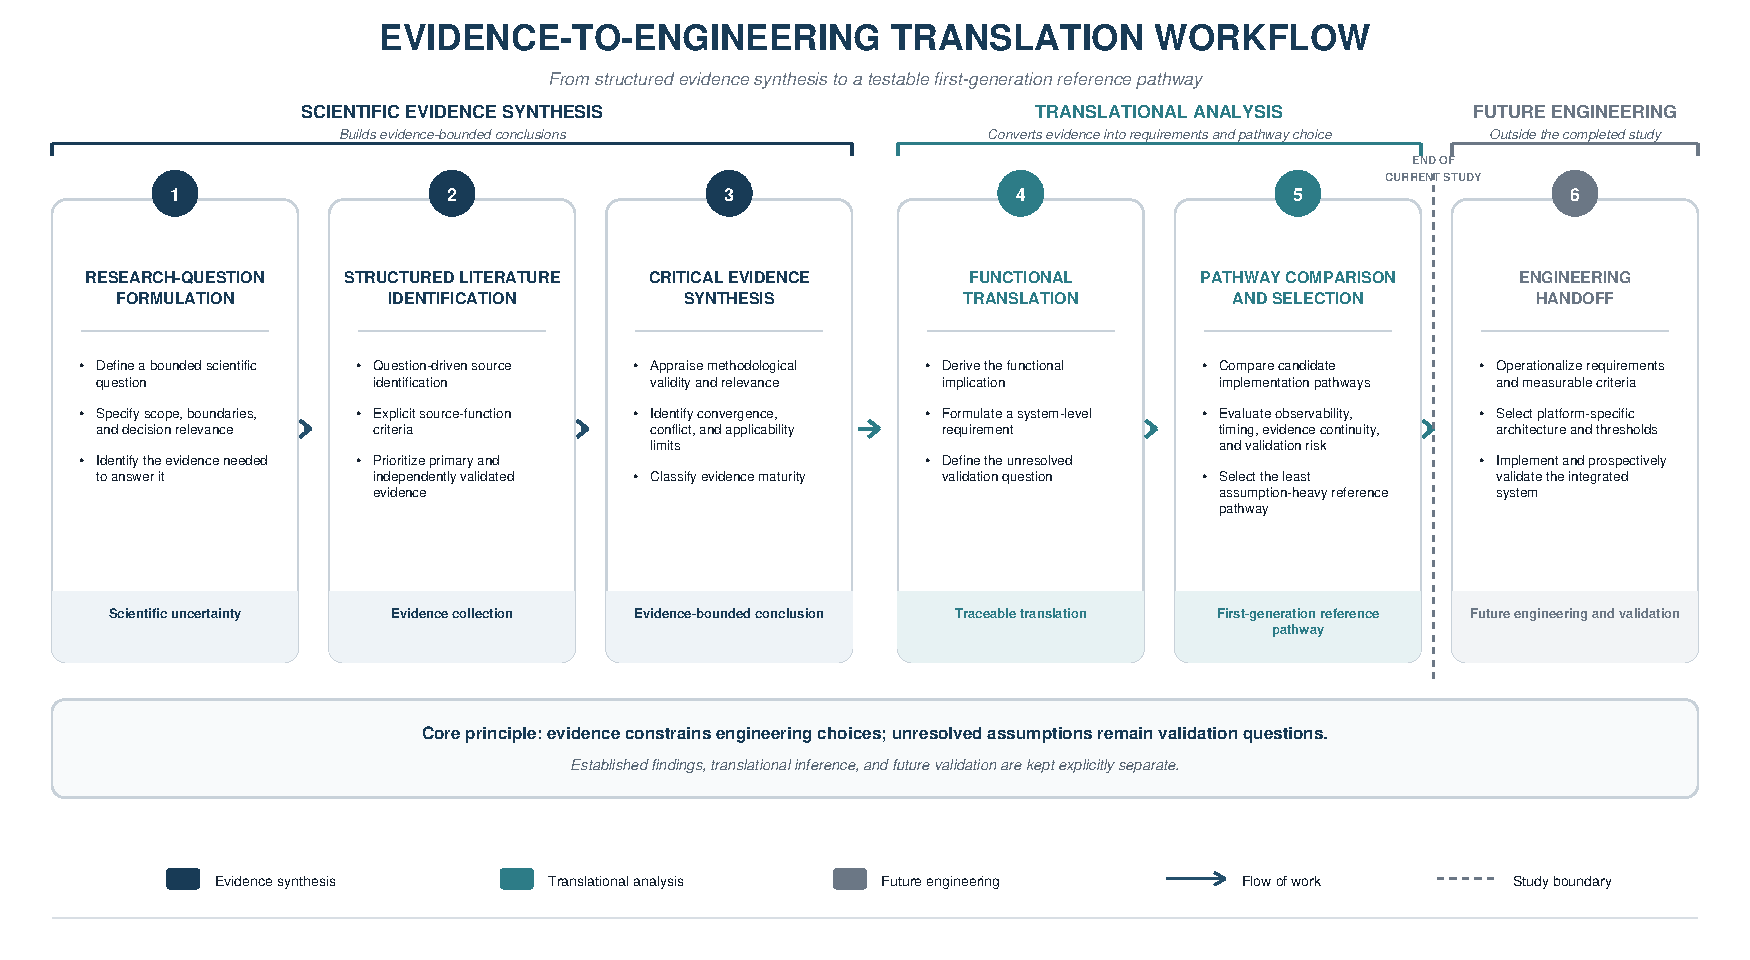
\includegraphics[width=\textwidth]
    {figures/fig1_research_workflow.pdf}
    \caption{
Evidence-to-engineering translation workflow used in this study.
Steps 1--3 formulate bounded research questions, identify relevant
literature through a structured question-driven process, and produce
evidence-bounded conclusions. Step~4 translates those conclusions into
functional implications, system-level requirements, and unresolved
validation questions. Step~5 compares candidate implementation pathways
and selects the first-generation reference pathway according to
physiological observability, evidentiary continuity, temporal suitability,
and validation risk. Step~6 represents the subsequent engineering and
prospective validation program and lies outside the completed scope of
the present study. Unresolved assumptions are retained as validation
questions rather than converted into predetermined engineering
specifications. The figure is an original methodological synthesis by
the author.
}
    \label{fig:research_workflow}
\end{figure*}

The six stages were:

\begin{enumerate}
    \item \textbf{Research-question formulation.}
    Each investigation began with a bounded question specifying the phenomenon,
    the evidence needed to evaluate it, and its relevance to the overall
    translation problem.

    \item \textbf{Structured literature identification.}
    Sources were selected according to their ability to establish a mechanism,
    quantify an effect, validate a measurement method, identify a limitation,
    or constrain a translational decision.

    \item \textbf{Critical evidence synthesis.}
    Findings were evaluated across studies to identify convergence,
    disagreement, applicability boundaries, methodological limitations, and
    unresolved uncertainty.

    \item \textbf{Functional translation.}
    Each evidence-bounded conclusion was reformulated as a statement of what a
    practical closed-loop system would need to accomplish.

    \item \textbf{Pathway comparison and selection.}
    Candidate implementation pathways were evaluated against the derived
    requirements according to physiological relevance, temporal suitability,
    evidence maturity, operational burden, and validation risk.

    \item \textbf{Engineering handoff.}
    The selected pathway and unresolved assumptions were transferred into a
    future program of component development, integration, prospective testing,
    and iterative refinement.
\end{enumerate}

The resulting requirement set covered seven areas:

\begin{itemize}
    \item \textbf{Physiological eligibility}: the states and conditions under
    which cueing may be appropriate;

    \item \textbf{Measurement quality}: the signal observability, reliability,
    physiological specificity, and uncertainty information required to support
    a decision;

    \item \textbf{Temporal validity}: the need for causal estimates, measurable
    processing delay, synchronized cue execution, and appropriately bounded
    intervention timing;

    \item \textbf{Intervention control}: the conditions under which cues must be
    delivered, withheld, modified, or terminated;

    \item \textbf{Disturbance prevention}: the detection and reduction of
    arousal, sleep disruption, inappropriate stimulation, or other unintended
    effects;

    \item \textbf{Operational reliability}: signal-quality monitoring,
    repeatability, fail-safe behavior, and robustness outside controlled
    laboratory conditions; and

    \item \textbf{Empirical validation}: the prospective tests required before
    an implementation assumption can be treated as a demonstrated capability.
\end{itemize}

Candidate pathways were evaluated according to how directly and reliably they
could satisfy these functions. Commercial availability, comfort, or
general-purpose sleep-staging performance were not sufficient grounds for
selection when the corresponding closed-loop function remained unsupported.
Where the evidence did not permit a definitive translation, uncertainty was
retained as a validation requirement rather than resolved through technological
preference.


\subsection{Study Outputs and Methodological Boundary}

The methodology produced four outputs:

\begin{enumerate}
    \item evidence-bounded conclusions concerning memory consolidation, TMR,
    wearable sensing, and closed-loop intervention;

    \item an evidence-derived set of system-level translational requirements;

    \item a structured comparison of candidate first-generation implementation
    pathways; and

    \item selection of the pathway with the strongest continuity with the
    established evidence and the fewest unsupported assumptions.
\end{enumerate}

These outputs define a scientifically justified starting point for subsequent
development. They do not constitute evidence that an integrated system has been
implemented, that its operating parameters have been determined, or that it
produces reliable memory benefits outside the conditions represented in the
reviewed literature.

The methodological conclusions are also bounded by the question-driven,
single-reviewer design. The synthesis did not provide exhaustive literature
retrieval, duplicate screening, formal risk-of-bias grading, or a new
meta-analysis. These limitations reduce the certainty with which the resulting
pathway can be generalized and are examined further in Section~7.

The present study therefore ends at pathway selection and qualitative
requirement definition. Subsequent work must operationalize the requirements,
select platform-specific architectures and thresholds, implement the
closed-loop system, and evaluate its physiological reliability, behavioral
efficacy, safety, and generalizability. The selected first-generation pathway
should be interpreted as a testable development hypothesis rather than as a
completed architecture or validated memory-enhancement product.

\section{Neuroscientific Foundations of Memory and Sleep}
\subsection{Neural Systems Relevant to Memory and Sleep}

The neurobiology relevant to Targeted Memory Reactivation (TMR) is distributed
across interacting memory, sensory, and sleep-regulatory systems. For the present
translation problem, the critical issue is not a complete account of human
neuroanatomy, but the relationship among three functions: the encoding and
reactivation of recently acquired memories, the regulation of sensory access
during sleep, and the maintenance of physiological states in which consolidation
can occur. These functions depend principally on hippocampal--neocortical,
thalamocortical, and sleep--wake regulatory networks
\citep{squire2015consolidation,scammell2017sleep}.

The hippocampus and distributed neocortical networks occupy complementary roles
in declarative memory. During learning, the hippocampus rapidly binds distributed
features of an experience represented across cortical regions, allowing recently
acquired information to be retrieved as an integrated memory. Over time,
reactivation of hippocampal--cortical representations is thought to contribute
to systems-level reorganization and integration with existing cortical knowledge
\citep{squire2015consolidation,dudai2015consolidation}. This process should not
be interpreted as a simple transfer from a temporary hippocampal store to a
permanent cortical store. The degree to which long-term memories become
independent of the hippocampus varies across memory types and remains the subject
of theoretical and empirical debate. For TMR, the important point is narrower:
recent memories can remain susceptible to post-encoding modification through
reactivation of distributed representations.

Sleep also changes how these memory systems interact with incoming sensory
information. The thalamus participates in state-dependent regulation of
thalamocortical communication and contributes directly to characteristic NREM
oscillations, particularly sleep spindles. Sensory transmission is attenuated
and reorganized during sleep rather than completely blocked, allowing the brain
to reduce responsiveness to much of the external environment while retaining
the capacity to process selected stimuli
\citep{scammell2017sleep,fernandez2020spindles}. This partial sensory
accessibility is essential to the biological plausibility of TMR: an external
cue must influence ongoing neural processing without producing sufficient
activation to destabilize sleep.

Hypothalamic and brainstem circuits contribute to the regulation and stability
of sleep--wake states, while structures including the amygdala can modulate the
salience and persistence of particular memories. These systems are relevant to
TMR primarily because they influence the physiological state in which cueing
occurs and the probability that sensory stimulation produces arousal rather
than memory-related processing. They are therefore treated here as modulatory
components of a larger network rather than as independent memory-storage systems
\citep{scammell2017sleep}.

\begin{figure*}[t]
    \centering
    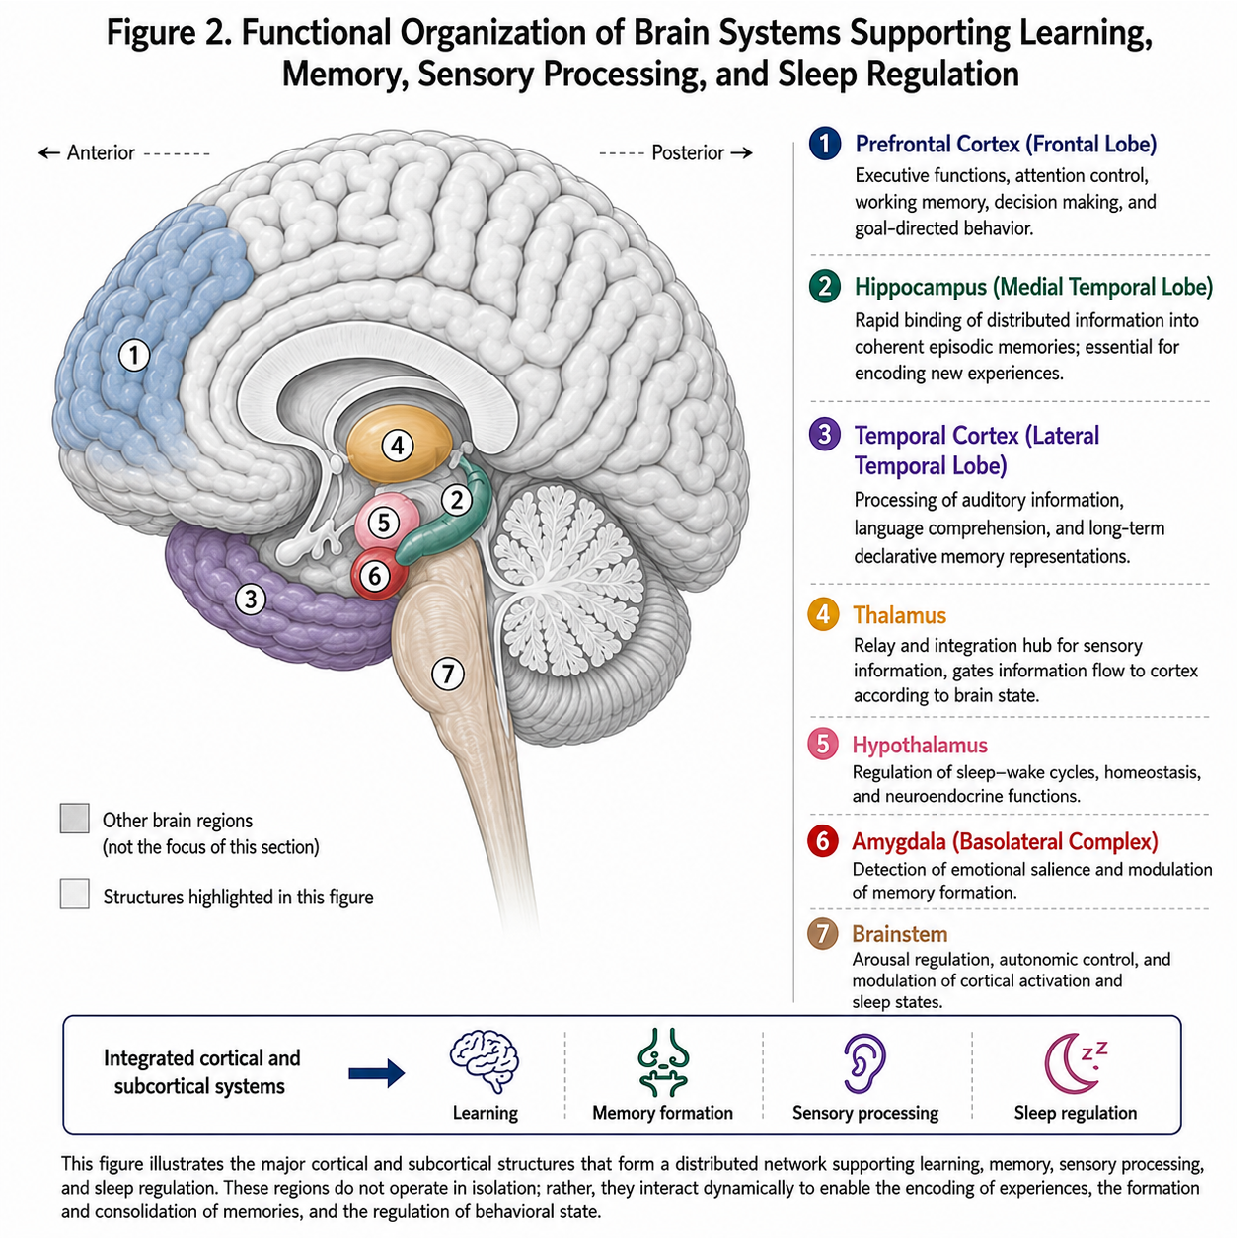
\includegraphics[width=\textwidth]
    {figures/fig2_memory_systems.pdf}
    \caption{
    Functional neural systems relevant to sleep-dependent memory processing.
    Hippocampal and distributed cortical networks support the encoding,
    reactivation, and longer-term reorganization of memory representations;
    thalamocortical circuits regulate state-dependent sensory processing and
    contribute to NREM oscillations; and hypothalamic and brainstem systems
    participate in sleep--wake and arousal regulation. The amygdala can
    additionally modulate memory according to emotional salience. The diagram
    represents a conceptual systems-level synthesis rather than anatomically
    independent functional modules
    \citep{squire2015consolidation,scammell2017sleep}.
    }
    \label{fig:functional_brain_systems}
\end{figure*}


\subsection{Electrophysiological Basis of Brain-State Monitoring}

For closed-loop TMR, the relevant bridge between neural physiology and
engineering is population-level electrophysiology. Information is transmitted
within and between neurons through electrical and chemical mechanisms, but
scalp-level measurements do not resolve individual neuronal communication.
Instead, coordinated activity across neuronal populations generates
extracellular electrical fields whose temporal structure can be measured at
progressively larger spatial scales.

Neural oscillations are recurring patterns of population activity produced by
interactions within and between neuronal circuits. They span multiple
frequencies and can organize the timing of neuronal excitability,
communication, and plasticity \citep{buzsaki2004oscillations}. Frequency bands
should not, however, be interpreted as one-to-one labels for specific cognitive
states. Multiple rhythms coexist, their properties vary across brain regions
and individuals, and their functional significance depends on the surrounding
physiological context. During sleep, several oscillatory events become
particularly informative because their occurrence and temporal relationships
change systematically across sleep states.

Electroencephalography (EEG) provides a non-invasive measurement of voltage
differences generated by these large-scale electrophysiological processes.
Scalp EEG is influenced primarily by coordinated transmembrane currents in
neuronal populations, particularly synaptic currents in spatially organized
cortical neurons, rather than by direct recording of individual action
potentials \citep{buzsaki2012origin}. EEG consequently provides high temporal
resolution but limited spatial specificity: it can reveal when large-scale
electrophysiological patterns occur without uniquely identifying the underlying
neuronal sources.

This distinction is important when EEG is used for sleep monitoring.
Conventional clinical sleep staging is based on polysomnography (PSG), which
combines EEG with electrooculography (EOG), electromyography (EMG), and other
physiological channels. Standard scoring assigns wake, N1, N2, N3, and REM
labels to successive epochs using characteristic combinations of these signals
\citep{silber2007scoring}. EEG contributes strongly to this classification,
particularly through changes in spectral activity and the appearance of events
such as K-complexes, sleep spindles, and slow waves, whereas rapid eye
movements are measured primarily by EOG and the reduction of skeletal-muscle
tone characteristic of REM sleep is assessed using EMG.

Conventional sleep-stage labels and the underlying electrophysiological events
also operate at different temporal scales. Manual staging is conventionally
performed over 30-s epochs, whereas slow waves, spindles, arousals, and other
transient events evolve over substantially shorter intervals
\citep{silber2007scoring}. A real-time intervention may therefore require more
than reproduction of conventional retrospective stage labels; it may also
require access to the continuous signal from which intervention-relevant events
and state transitions can be detected.

A further measurement boundary is particularly important for the later
engineering analysis. Cortical slow waves and sleep spindles are observable in
scalp EEG, whereas hippocampal sharp-wave ripples are primarily characterized
through intracranial recordings and are not directly available from ordinary
wearable scalp EEG. Human intracranial studies nevertheless show temporal
coordination among hippocampal ripples, sleep spindles, and slow oscillations
\citep{staresina2015nesting}. Accordingly, hippocampal ripple activity can
inform the biological model of sleep-dependent consolidation without being
treated as a directly measurable control signal in a first-generation wearable
EEG system.

\begin{figure*}[t]
    \centering
    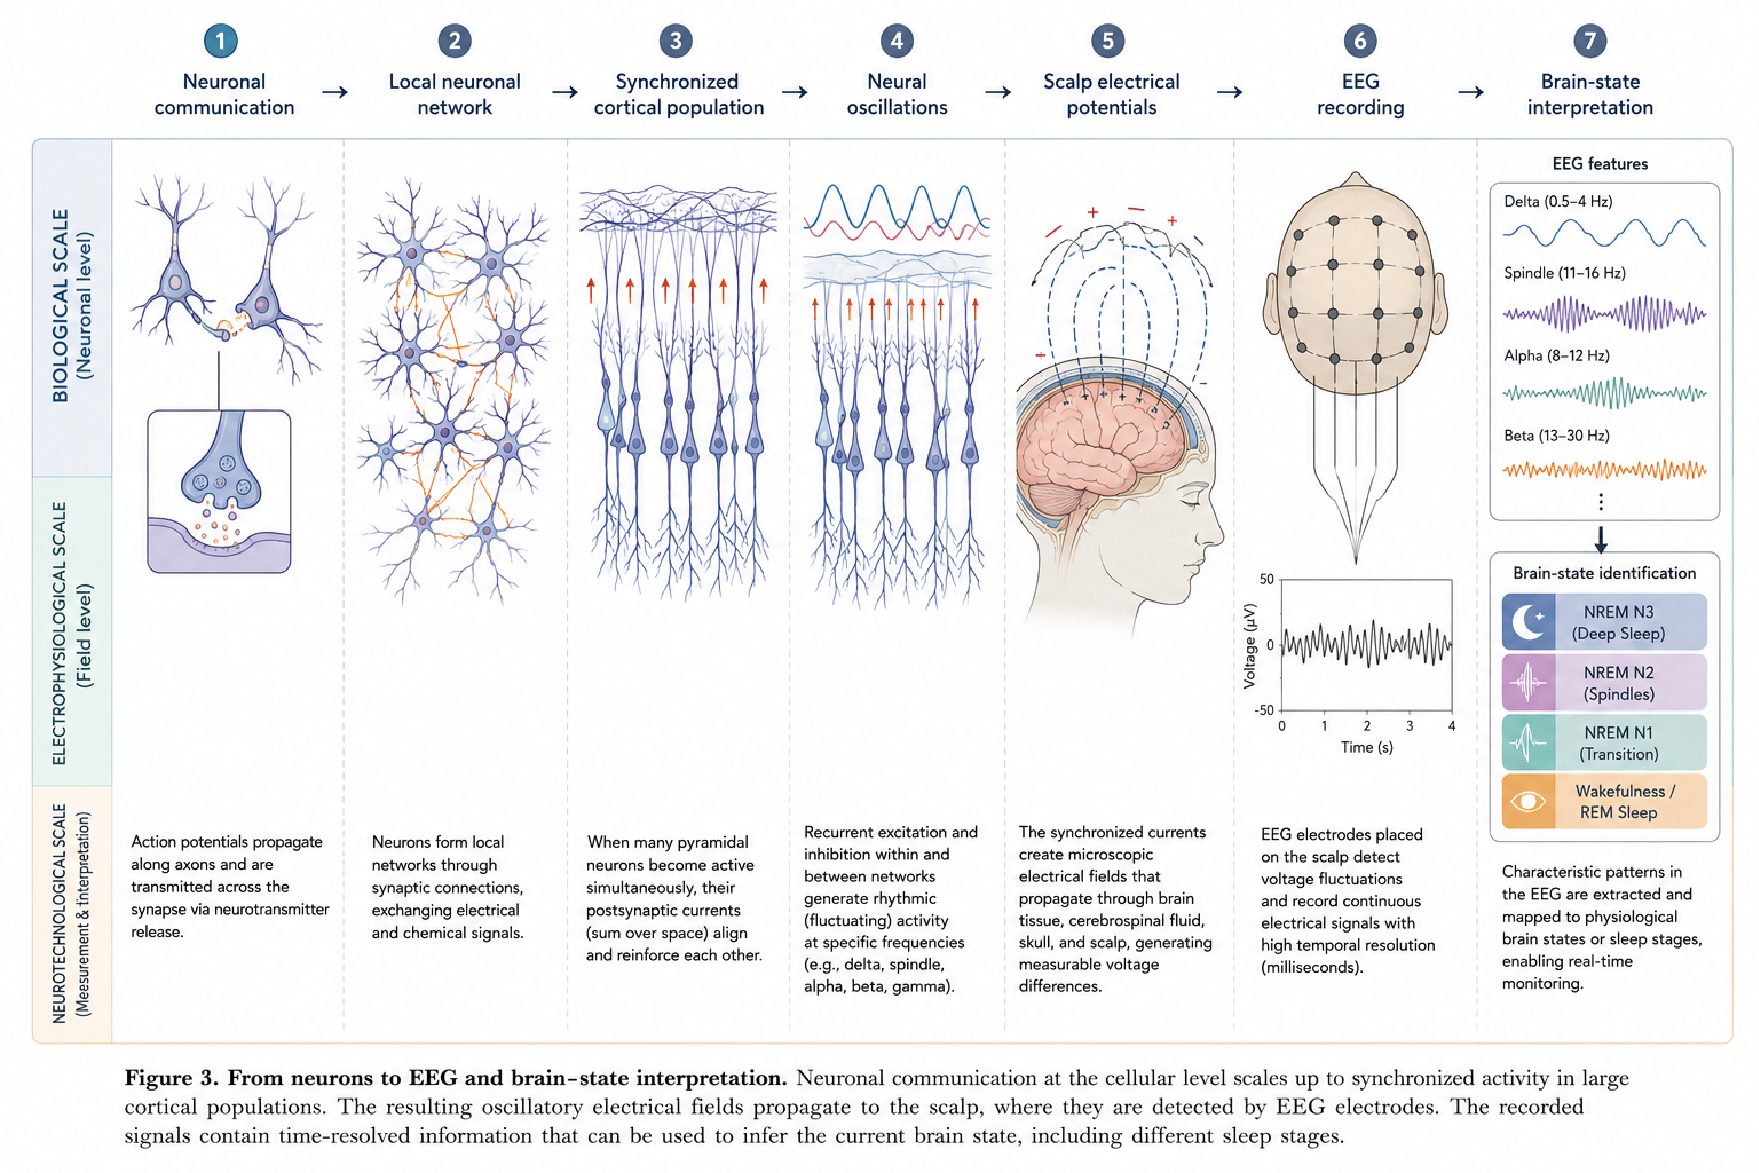
\includegraphics[width=\textwidth]
    {figures/fig3_neurons_to_EEG.pdf}
    \caption{
    Conceptual relationship between neuronal population activity and
    EEG-based brain-state interpretation. Coordinated transmembrane currents
    across neuronal populations generate extracellular fields that contribute
    to measurable scalp potentials. Their temporal organization produces EEG
    features, including oscillatory activity and transient events, that can be
    used as physiological indicators of sleep state. Scalp EEG reflects
    population-level activity and does not directly record individual neurons
    or deep hippocampal sharp-wave ripples
    \citep{buzsaki2012origin}.
    }
    \label{fig:neurons-to-eeg}
\end{figure*}


\subsection{Memory Consolidation and Reactivation}

Encoding does not immediately produce a fixed long-term memory. Newly acquired
representations remain susceptible to interference and modification, and their
persistence depends on biological processes collectively described as memory
consolidation. Consolidation operates across multiple temporal and spatial
scales, from cellular and synaptic modifications within initially engaged
circuits to systems-level changes in how memories are represented across
hippocampal and cortical networks
\citep{squire2015consolidation,dudai2015consolidation}.

Synaptic consolidation refers broadly to post-learning cellular processes that
stabilize experience-dependent changes within local circuits. Systems
consolidation concerns longer-term reorganization of distributed memory
representations and changes in interactions between the hippocampus and
neocortex. These processes should not be treated as a single linear transfer
mechanism: their time courses overlap, their expression depends on the type of
memory, and multiple theoretical accounts differ in the extent to which remote
memories continue to require hippocampal involvement
\citep{squire2015consolidation,dudai2015consolidation}.

A central process linking learning to later systems-level change is memory
reactivation. Neural patterns related to previous experience can reappear after
encoding during both wakefulness and sleep. During NREM sleep, such
reactivation is frequently observed in temporal association with hippocampal
sharp-wave ripples and with cortical and thalamocortical oscillations implicated
in memory processing \citep{rasch2013sleep,klinzing2019mechanisms}. Reactivation
is therefore widely considered an important component of contemporary models
of sleep-dependent systems consolidation.

The mechanistic interpretation nevertheless requires caution. Reactivation is
not synonymous with consolidation, and the occurrence of replay-like activity
does not imply that every reactivation event strengthens a memory. Instead,
reactivation provides an opportunity for previously encoded representations to
be modified, integrated, or stabilized under physiological conditions that
support plasticity. The behavioral consequences depend on the memory,
surrounding neural state, and temporal organization of the relevant activity
\citep{dudai2015consolidation,klinzing2019mechanisms}.

This distinction is central to TMR. A sensory cue presented during sleep cannot
be assumed to create or restore a memory that was not successfully encoded.
Rather, TMR depends on an association established during wakefulness and seeks
to bias subsequent reactivation toward the corresponding representation. The
scientific target of the intervention is therefore an endogenous post-encoding
process, not memory formation independently of prior learning.


\subsection{Sleep Architecture and Oscillatory Coordination of Memory}

Human sleep is organized into recurring transitions among NREM and REM states.
Under contemporary clinical scoring conventions, NREM sleep is divided into
N1, N2, and N3. N1 represents the transition from wakefulness into sleep; N2 is
characterized in part by K-complexes and sleep spindles; and N3 contains
prominent high-amplitude slow-wave activity and is commonly referred to as
slow-wave sleep (SWS) in human experimental research. REM sleep differs from
NREM sleep through a combination of relatively low-amplitude mixed-frequency
EEG activity, rapid eye movements, and reduced skeletal-muscle tone
\citep{silber2007scoring}.

These stages should not be interpreted as discrete functional compartments in
which a single cognitive process occurs exclusively. Memory-related processing
is distributed across the sleep period, and different forms of learning can
show different relationships with NREM and REM physiology
\citep{diekelmann2010memory,rasch2013sleep}. For the declarative memory
processes most relevant to much of the TMR literature, NREM sleep---particularly
N2 and N3---provides a well-supported physiological context for examining
reactivation and hippocampal--neocortical communication. This does not imply
that N3 is universally optimal for every memory domain or cueing protocol.

A prominent mechanistic framework for NREM-dependent systems consolidation
centers on the temporal coordination of cortical slow oscillations,
thalamocortical sleep spindles, and hippocampal sharp-wave ripples. Slow
oscillations organize alternating periods of cortical excitability; spindles
emerge from thalamocortical circuitry and are associated with transient windows
of cortical plasticity; and hippocampal sharp-wave ripples are closely
associated with replay of recently experienced activity. Converging evidence
suggests that their temporal nesting can support communication between
hippocampal and cortical memory systems
\citep{staresina2015nesting,fernandez2020spindles,klinzing2019mechanisms}.

The coupling of these events is scientifically important but should not be
converted prematurely into a requirement for phase-specific stimulation.
Evidence that oscillatory coordination contributes to consolidation does not,
by itself, establish that a first-generation TMR system must detect every event
or deliver cues at a particular oscillatory phase. Stage-aware cueing and
event- or phase-aware cueing therefore represent distinct levels of
intervention control. Whether the additional temporal precision of the latter
produces a reproducible behavioral advantage is an empirical question addressed
later in the translational analysis.

For wearable implementation, this distinction also separates the biological
mechanism from what can actually be observed. Scalp EEG can provide information
about sleep stage, cortical slow-wave activity, and sleep spindles, while deeper
hippocampal processes remain indirectly inferred. The relevant engineering
question is consequently not whether every component of the consolidation
mechanism can be measured non-invasively, but whether the observable signals
provide sufficient information to identify physiologically appropriate
conditions for intervention.

\begin{figure*}[t]
    \centering
    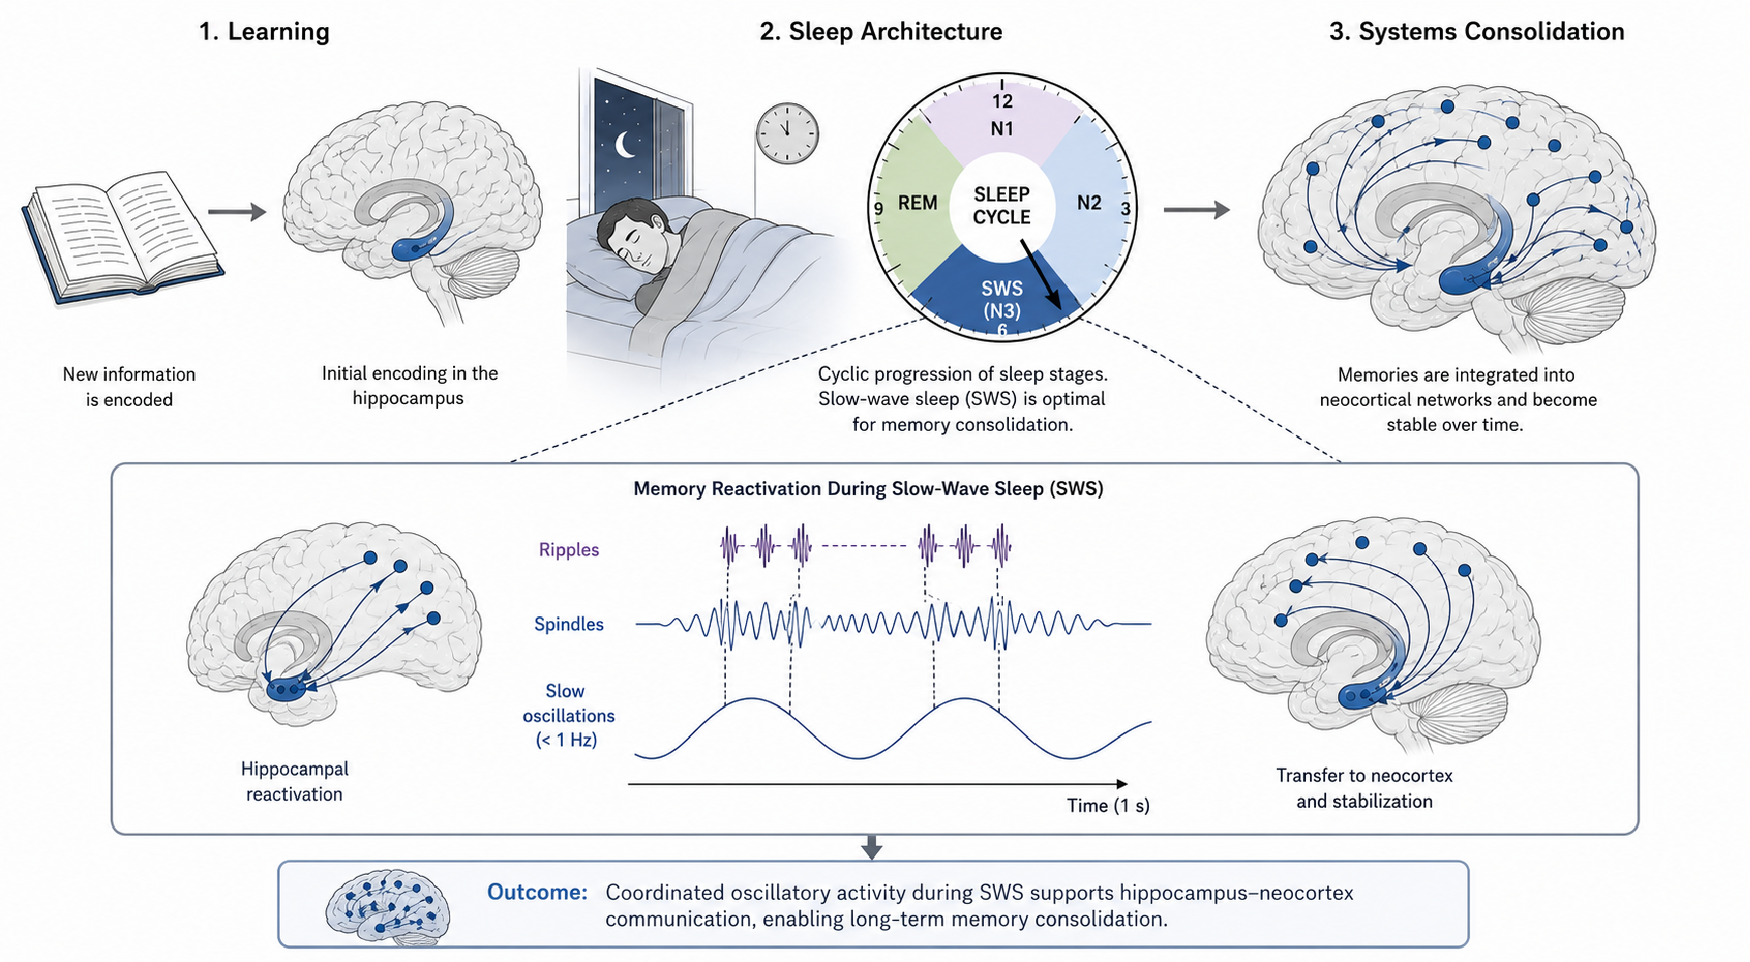
\includegraphics[width=\textwidth]
    {figures/fig4_sleep_dependent_consolidation.pdf}
    \caption{
    Conceptual framework of sleep-dependent systems memory consolidation.
    Recently encoded memories initially depend strongly on interactions between
    hippocampal and distributed cortical representations. During NREM sleep,
    memory reactivation occurs within a physiological environment characterized
    by coordinated cortical slow oscillations, thalamocortical sleep spindles,
    and hippocampal sharp-wave ripples. Their temporal interaction is proposed
    to support communication and longer-term reorganization across memory
    networks. The figure represents a mechanistic synthesis rather than a
    claim that consolidation proceeds through a single deterministic pathway
    \citep{rasch2013sleep,staresina2015nesting,klinzing2019mechanisms}.
    }
    \label{fig:sleep-dependent-consolidation}
\end{figure*}

Together, these findings establish the biological constraints relevant to TMR:
a previously encoded representation must remain capable of reactivation, cueing
must occur within an appropriate physiological state, and the intervention must
preserve rather than disrupt the sleep processes associated with consolidation.
Section~4 examines the extent to which experimental TMR can exploit these
conditions to produce measurable changes in subsequent memory.

\section{Targeted Memory Reactivation: From Biological Mechanism to Closed-Loop Intervention}
\subsection{Experimental Principle of Targeted Memory Reactivation}

Targeted Memory Reactivation (TMR) is an experimental procedure for biasing
post-encoding memory processing through sensory cues associated with prior
learning. During wakefulness, a sound, odor, or other stimulus is paired with
specific learned information. Re-presentation of that cue during subsequent
sleep can selectively influence later retention of the associated material
\citep{rasch2007odor,rudoy2009strengthening,oudiette2013upgrading}. TMR
therefore does not introduce information into memory during sleep; it acts on
representations established before sleep by providing an external signal linked
to the earlier learning episode.

The mechanistic interpretation of this effect requires caution. A selective
behavioral benefit following cueing is evidence that the cue altered
post-encoding memory processing, but it does not by itself demonstrate the
precise neural content or pathway of reactivation. Neuroimaging and
electrophysiological studies provide additional evidence that sleep-time cues
can evoke learning-related activity and content-specific neural patterns
\citep{rasch2007odor,cairney2018spindle,wang2019signals}. The most defensible
interpretation is therefore that appropriately associated cues can bias
endogenous memory reactivation during sleep, while the exact neural sequence
linking cue perception to later behavioral improvement remains incompletely
resolved.

This distinction separates TMR from nonspecific sensory stimulation. Its
experimental logic depends on three linked conditions: the existence of a
pre-sleep cue--memory association, presentation of the cue under an appropriate
physiological condition, and a subsequent difference in memory attributable to
the cueing manipulation. These conditions form the basis for evaluating both
TMR efficacy and its later translation into an automated intervention.


\subsection{Encoding and Cue--Memory Association}

The effectiveness of TMR is constrained by what has been learned before sleep.
A cue can only influence a memory insofar as it has acquired a meaningful
relationship with the target representation during encoding. Evidence from
object--location and associative-learning paradigms indicates that prior memory
strength and the directness of the cue--memory association can influence the
magnitude of subsequent TMR effects
\citep{creery2015priorlearning,cairney2016benefits}.

This relationship is more nuanced than a simple requirement for maximally strong
encoding. Creery et al.\ found that near-perfectly learned spatial memories did
not show the same TMR benefit as less completely learned memories, while Cairney
et al.\ reported stronger effects for memories recalled with relatively low
pre-sleep accuracy and found evidence that direct cue--memory associations were
important for successful reactivation
\citep{creery2015priorlearning,cairney2016benefits}. TMR should therefore not
be described as rescuing memories that were never encoded, but neither should
weak pre-sleep performance automatically be treated as a failure condition.

Cue specificity also affects interpretation. Item-specific auditory cues can
permit selective comparison between cued and uncued memories, as demonstrated
by Rudoy et al., whereas contextual cues such as odors can reactivate a broader
learning context \citep{rasch2007odor,rudoy2009strengthening}. Behavioral
selectivity should not be equated with complete neural isolation: a cue may
reactivate features of the target memory together with contextual or associated
representations. For translational purposes, the critical requirement is
therefore not maximal cue uniqueness in the abstract, but a reproducible
association between the cue and the memory process the intervention is intended
to influence.


\subsection{Physiological Conditions for State-Dependent Cueing}

TMR efficacy depends not only on what is cued, but also on the physiological
state in which cueing occurs. The meta-analysis by Hu et al.\ found significant
positive effects for cueing during NREM stage~2
(\(g=0.32\), 95\% CI \(0.04\)--\(0.60\)) and slow-wave sleep
(\(g=0.27\), 95\% CI \(0.20\)--\(0.35\)), whereas pooled effects for REM sleep
and wakefulness were not significant
\citep{hu2020promoting}. These results support NREM sleep as the best-established
cueing context in the literature synthesized by that analysis, but they do not
establish that a single sleep stage is universally optimal for every memory
domain or experimental objective.

The physiological context described in Section~3 provides a plausible basis for
this state dependence. During NREM sleep, slow oscillations, sleep spindles, and
hippocampal activity associated with memory reprocessing exhibit structured
temporal relationships
\citep{rasch2013sleep,klinzing2019mechanisms,staresina2015nesting}. TMR cues
enter this ongoing physiological environment rather than initiating
consolidation independently. Accordingly, cue timing should be understood as an
interaction with endogenous sleep dynamics rather than as delivery of a stimulus
to a uniformly receptive sleeping brain.

Evidence also indicates that finer temporal structure within NREM can influence
cue efficacy. Cue-induced spindle activity has been associated with successful
memory processing, and manipulation of cue timing relative to spindle dynamics
has demonstrated that some NREM intervals are more favorable than others
\citep{cairney2018spindle,antony2018spindle}. More direct closed-loop evidence
has subsequently tested TMR relative to ongoing slow-oscillation phase.
Shimizu et al.\ implemented an EEG-based closed-loop system that delivered
memory-associated sounds around detected slow-oscillation down-to-up
transitions and reported improved spatial-navigation performance relative to a
non-stimulated control condition \citep{shimizu2018closedloop}. The study
demonstrated the feasibility and behavioral relevance of phase-sensitive
closed-loop TMR, although it did not establish superiority over an otherwise
equivalent open-loop TMR protocol.

Ngo and Staresina later directly compared memory cues delivered during
slow-oscillation UP and DOWN states and found reduced overnight forgetting for
memories cued during UP states relative to DOWN states
\citep{ngo2022shaping}. More recently, Nicolas et al.\ extended this approach
to motor memory and likewise found phase-dependent behavioral and
electrophysiological effects, with greater overnight performance improvement
for UP- than DOWN-reactivated motor sequences
\citep{nicolas2025phase}. Importantly, the UP-reactivated condition in that
study did not significantly outperform the non-reactivated condition,
illustrating that evidence for phase dependence does not yet establish a
general incremental advantage of phase-locked TMR over simpler cueing
strategies.

These findings provide direct empirical support for event- and phase-aware
closed-loop TMR rather than merely a mechanistic rationale for it. The evidence
base is nevertheless narrower than that supporting TMR delivered within broader
NREM conditions, and phase-specific control introduces additional requirements
for causal event detection, phase estimation, synchronization, and cue timing.
Stage-aware and phase-aware control should therefore remain distinct levels of
intervention complexity.

These findings provide the rationale for state-dependent closed-loop control in
an autonomous implementation. TMR itself does not require an automated
closed-loop system; many foundational studies relied on experimenter-supervised
sleep monitoring. For real-world automation, however, physiological information
must replace continuous researcher judgment. Such a system must determine when
cueing is permitted, when it should be withheld, and when evidence of disturbance
should interrupt further stimulation. The quantitative thresholds and algorithms
needed to implement these functions remain engineering and validation questions
rather than established neuroscientific constants.


\begin{figure*}[t]
    \centering
    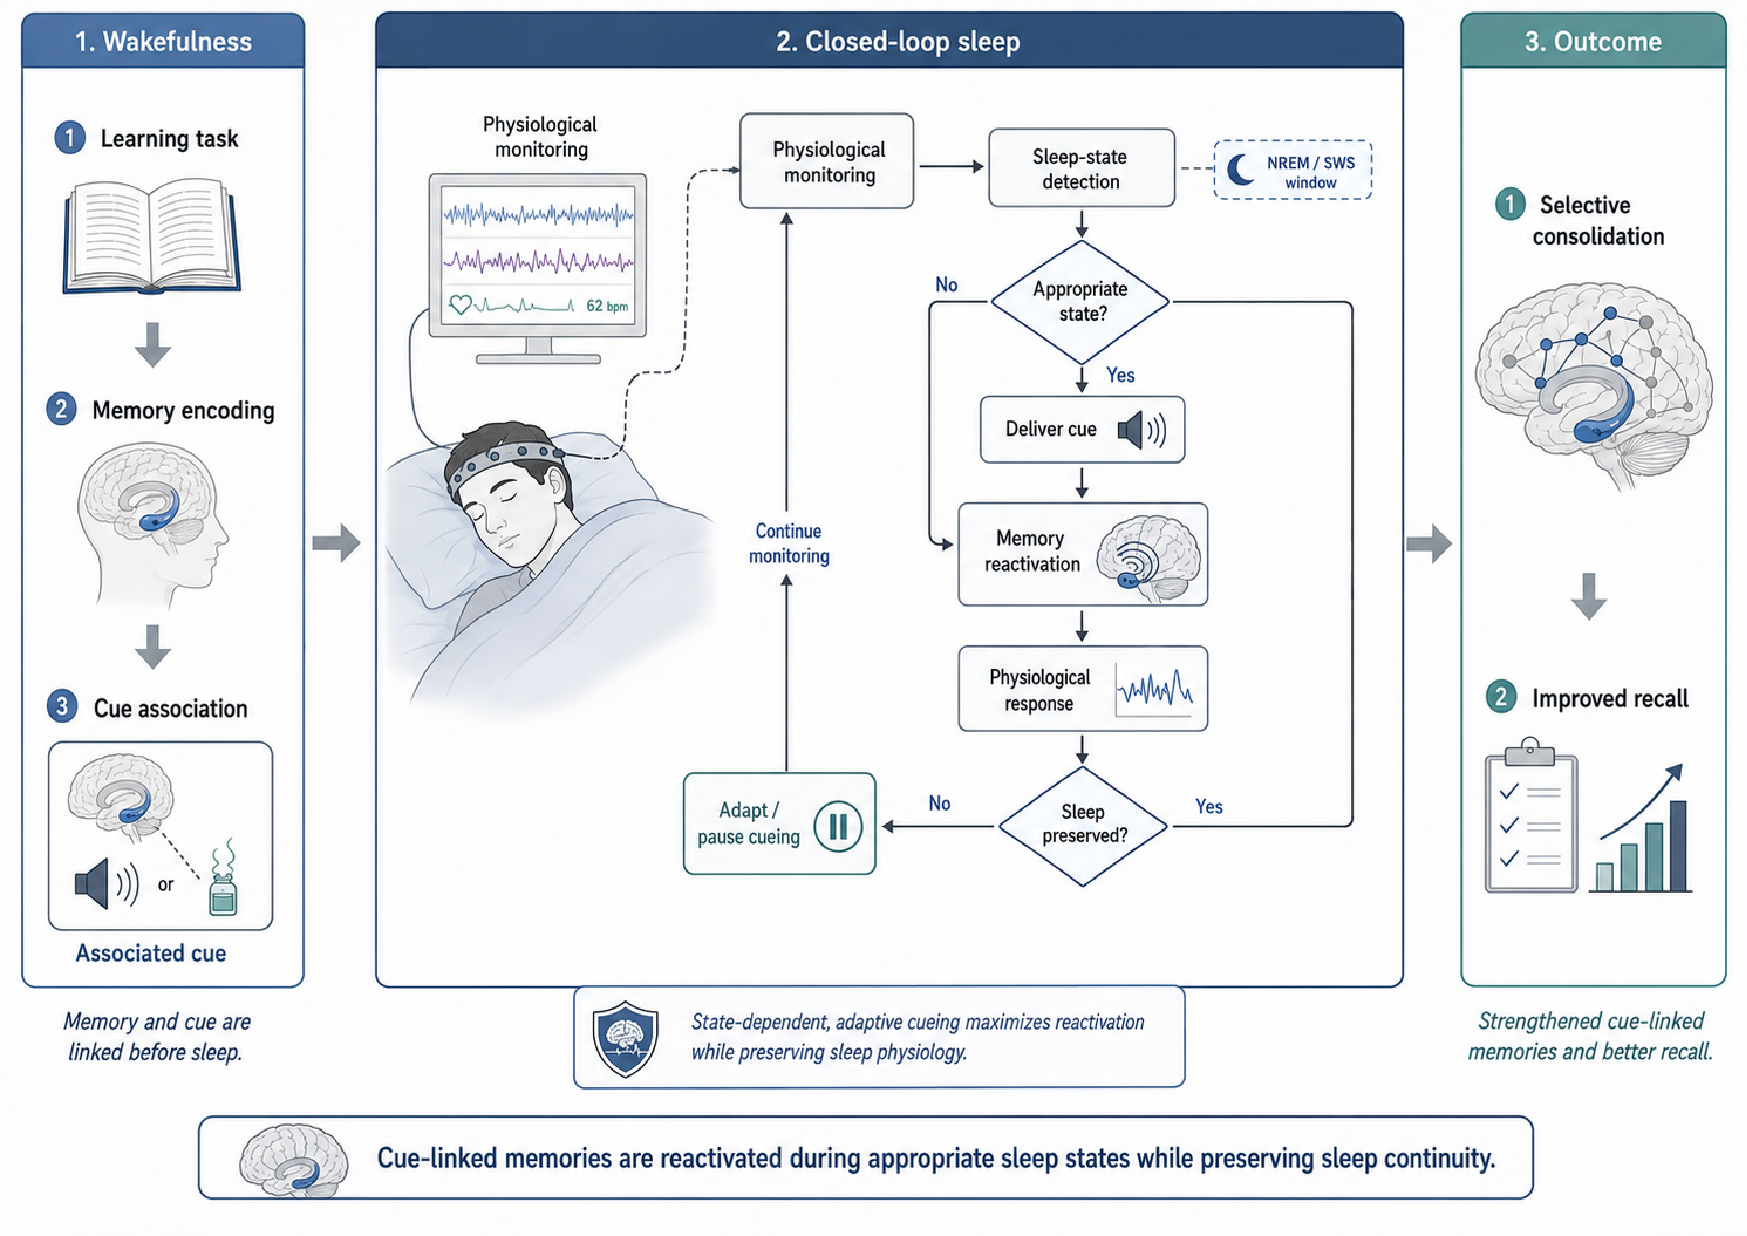
\includegraphics[
        width=\textwidth,
        keepaspectratio
    ]{figures/fig5_TMR_closed_loop.pdf}

    \caption{
    Conceptual workflow for state-dependent closed-loop Targeted Memory
    Reactivation. Sensory cues are first associated with selected information
    during wakeful learning. During subsequent sleep, ongoing physiological
    measurements are used to determine whether the current state is eligible
    for cue presentation. Following stimulation, physiological information can
    be used to evaluate disturbance and determine whether cueing should continue,
    be delayed, or be suspended. The workflow is an original conceptual
    synthesis of experimental and automated TMR paradigms; cue delivery does not
    guarantee memory enhancement, and behavioral efficacy remains an empirical
    outcome
    \citep{oudiette2013upgrading,whitmore2022improving,salfi2025promoting}.
    }
    \label{fig:tmr_closed_loop_process}
\end{figure*}


\subsection{Experimental Evidence for TMR Efficacy and Mechanism}

Early controlled experiments established the fundamental causal effect of
sleep-time cue presentation on later memory performance. Rasch et al.\
re-presented an odor that had been present during learning and found improved
retention of a hippocampus-dependent spatial task when the odor was presented
during slow-wave sleep. The same manipulation was ineffective when the odor had
not been associated with learning and did not produce the corresponding benefit
during wakefulness or REM sleep
\citep{rasch2007odor}. The experiment therefore demonstrated that the behavioral
effect depended jointly on prior association and physiological state rather than
on sensory stimulation alone.

Rudoy et al.\ subsequently demonstrated item-level selectivity using an
object--location task. Individual objects were paired with characteristic sounds
during learning, and only a subset of those sounds was replayed during sleep.
Post-sleep location memory was more accurate for cued than uncued objects
\citep{rudoy2009strengthening}. Because cued and uncued items were learned by
the same individuals and experienced the same sleep period, this within-subject
design provided strong evidence that targeted sensory reminders can alter the
retention of selected memories.

The broader magnitude of the effect was quantified by Hu et al.\ in a multilevel
meta-analysis of 91 experiments, 212 effect sizes, and 2,004 participants.
Across sleep-based TMR experiments, the pooled effect was
Hedges' \(g=0.29\) (95\% CI \(0.21\)--\(0.38\))
\citep{hu2020promoting}. This represents a modest standardized benefit, not a
29\% improvement in memory performance and not an expected effect for every
participant or protocol.

The same meta-analysis also places an important boundary around that estimate.
Effect sizes were substantially heterogeneous
(\(I^2=71\%\)), indicating large variation beyond sampling error. Hu et al.\
also detected funnel-plot asymmetry consistent with possible publication bias;
under one trim-and-fill correction, the estimated overall effect decreased to
\(g=0.18\) (95\% CI \(0.06\)--\(0.30\)) while remaining significantly above
zero \citep{hu2020promoting}. The central quantitative conclusion is therefore
not that TMR produces a fixed effect of \(g=0.29\), but that the literature
supports a small positive average effect whose magnitude is strongly
condition-dependent.

Neurophysiological findings provide convergent but not definitive evidence about
the mechanism underlying this behavioral effect. Cairney et al.\ found that
memory cues increased fast-spindle activity relative to control stimuli and
that memory-category information could be decoded during this spindle response;
the fidelity of decoding predicted later TMR benefit
\citep{cairney2018spindle}. Wang et al.\ likewise identified
content-related EEG activity following sleep-time cues, with stronger
learning-related signals associated with subsequent memory and post-cue spindle
activity \citep{wang2019signals}. Antony et al.\ further showed that
experimentally manipulating cue timing relative to ongoing spindle dynamics
changed later memory performance \citep{antony2018spindle}.

These studies strengthen the interpretation that TMR can engage
memory-specific processing embedded within NREM electrophysiology. They do not,
however, justify treating any single EEG response as a validated surrogate for
successful memory enhancement. Spindle activity and decodable neural patterns
are mechanistically informative, but their relationship to behavioral benefit
remains variable and in several studies correlational. Behavioral outcome
therefore remains necessary when evaluating TMR efficacy.


\subsection{From Laboratory Demonstration to Home-Based Feasibility}

Moving TMR beyond supervised laboratory environments introduces a different
evidentiary question: whether the intervention can preserve its physiological
and behavioral properties when monitoring and cue delivery are automated.
Early unsupervised work demonstrated the difficulty of this transition.
G{\"o}ldi and Rasch applied vocabulary cueing across three nights at home without
online sleep-state control and found no uniform benefit across the full sample;
outcomes depended strongly on reported sleep disturbance and habituation
\citep{goldi2019home}. This result is important because it shows that removing
physiological supervision does not automatically preserve laboratory efficacy.

Whitmore et al.\ subsequently developed SleepStim, which combined smartwatch
movement and heart-rate measurements with a smartphone-based auditory cueing
system. In the first experiment (\(n=61\)), the overall TMR effect was not
significant, although memory outcome varied systematically with sound intensity.
After restricting stimulus intensity in a second experiment (\(n=24\)), cued
spatial memories showed a significant advantage
\citep{whitmore2022improving}. The study provides evidence that automated
peripheral-sensor-guided TMR can operate at home while simultaneously
demonstrating that intervention parameters and sleep disturbance materially
affect the result.

More direct electrophysiological control was demonstrated by Salfi et al.\ using
a Dreem~2 wearable EEG system in 24 adults sleeping at home. Participants
learned translations for 40 pseudowords, half of which were subsequently
re-presented following real-time detection of slow waves. Cued items improved
by 8.6\% from evening test to morning retest, whereas the corresponding change
for uncued items was not significant; morning recall was also higher for cued
than uncued material. Successful recall was associated with greater
post-stimulus spindle-range activity
\citep{salfi2025promoting}.

Taken together, these studies provide proof-of-concept evidence for automated
home TMR across both peripheral and EEG-based sensing approaches
\citep{goldi2019home,whitmore2022improving,salfi2025promoting}. They do not
establish population-level effectiveness, long-term reliability, or equivalence
between sensing modalities. The evidence instead demonstrates a progression
from unsupervised cue playback to physiological state-dependent automation,
while showing that sensing quality, stimulation control, and preservation of
sleep remain central determinants of translational success.


\subsection{Boundary Conditions and Evidence-Derived Implications}

TMR should therefore be interpreted as a condition-dependent intervention rather
than a deterministic memory-enhancement mechanism. Its pooled behavioral effect
is positive but modest, and substantial between-study heterogeneity indicates
that protocol, memory type, sleep state, and participant-level factors materially
influence outcome \citep{hu2020promoting}. Prior memory strength and the
structure of cue--memory associations provide additional sources of variability
\citep{creery2015priorlearning,cairney2016benefits}.

Individual predictability remains particularly limited. Differences in sleep
architecture, sensory threshold, initial learning, cue responsiveness, and
oscillatory physiology may contribute to variation between participants and
nights, but currently available neural markers should not be treated as
prospectively validated predictors of individual benefit. A strong cue-evoked
spindle response can be associated with successful memory processing without
guaranteeing that a specific memory will subsequently improve.

The durability and generalization of TMR effects also remain incompletely
characterized. Much of the evidence relevant to the present synthesis measures
memory over relatively short post-sleep intervals, while only limited work has
examined repeated unsupervised use across multiple nights
\citep{goldi2019home,whitmore2022improving}. Evidence that TMR improves a
specific cued memory should therefore not be generalized to durable cognitive
enhancement, broad learning improvement, or cumulative benefits from indefinite
repeated stimulation.

Mechanistic uncertainty likewise remains relevant to intervention design.
Cue-evoked spindle activity, content-specific neural decoding, and temporal
sensitivity to oscillatory state support contemporary reactivation models
\citep{cairney2018spindle,wang2019signals,antony2018spindle}, but they do not
yet establish a single optimal triggering rule. In particular, evidence that
fine-scale oscillatory timing influences TMR should not be converted directly
into a requirement for phase-specific first-generation control. Whether
event-aware or phase-aware cueing provides a reproducible advantage over
well-controlled stage-aware TMR remains an empirical comparison.

The evidence reviewed in this section nevertheless establishes several
translational constraints. A practical TMR system must operate on memories that
have been associated with recoverable cues before sleep; cueing must be limited
to physiologically supported sleep conditions; stimulation must be controlled
to reduce sleep disturbance; and intervention timing and physiological context
must be recorded so that behavioral outcomes can be interpreted in relation to
actual system operation. These conclusions define the biological requirements
of the intervention without determining which sensing technology can satisfy
them. Section~5 therefore evaluates the wearable measurement pathways available
for observing those conditions in real time.

\section{Wearable Sleep Monitoring}
\subsection{Polysomnography and the Physiological Measurement Target}

Polysomnography (PSG) provides the reference framework for characterizing human
sleep because sleep stages are defined from multiple physiological signals rather
than from behavior or movement alone. Standard PSG combines
electroencephalography (EEG), electrooculography (EOG), and electromyography
(EMG), with additional respiratory and cardiovascular channels included when
required. Under conventional scoring rules, these signals are interpreted
together to classify successive 30-s epochs as wake, N1, N2, N3, or rapid eye
movement (REM) sleep \citep{silber2007scoring}.

For TMR, the relevance of PSG extends beyond the categorical stage label. EEG
also preserves information about transient electrophysiological events such as
slow waves, sleep spindles, K-complexes, and cortical arousals. These events can
occur at substantially shorter timescales than the epochs used for conventional
sleep staging. A recording may therefore be correctly classified as N2 or N3
while still containing moment-to-moment physiological variation relevant to
whether stimulation should occur.

PSG should nevertheless be treated as a standardized reference rather than as
an error-free representation of a continuously evolving brain state. Human sleep
scoring contains genuine ambiguity, particularly near stage transitions.
Rosenberg and Van Hout reported an average inter-scorer stage agreement of
82.6\% in the American Academy of Sleep Medicine inter-scorer program, with
lower agreement for N3 and especially N1 than for several other stages
\citep{rosenberg2013interscorer}. Wearable performance should consequently be
interpreted relative to a high-quality physiological reference whose own
categorical labels contain uncertainty.

The translational objective is therefore not to reproduce the complete PSG
laboratory in wearable form. It is to determine which components of the
physiological information available in PSG must remain observable for a
particular closed-loop decision. This distinction permits reduced sensing
systems to be evaluated according to functional adequacy rather than according
to whether they reproduce every channel used in clinical polysomnography.


\subsection{Wearable EEG: Preserving Electrophysiological Observability}

Wearable EEG attempts to preserve access to scalp electrophysiology while
reducing the recording burden of full PSG. Compared with peripheral sensing,
its principal scientific advantage is not that it measures sleep ``directly,''
but that the recorded signal contains electrophysiological features from which
sleep stages and several intervention-relevant events are conventionally
defined. Depending on montage and signal quality, wearable EEG may preserve
information about slow-wave activity, sleep spindles, stage transitions, and
cortical responses to sensory stimulation.

Reducing the number of electrodes introduces important trade-offs. Fewer
channels reduce spatial coverage and redundancy and may make it more difficult
to distinguish localized artifact from genuine physiology. They do not,
however, inherently remove EEG's high temporal resolution. The relevant
question is whether a particular montage preserves the signal features required
by the intended decision and whether those features remain reliable throughout
overnight use.

Empirical validation demonstrates both the potential and the limitations of
this approach. In a developer-associated validation of the Dreem headband,
Arnal et al.\ compared simultaneous headband and PSG recordings in 25
participants. Automatic sleep staging achieved a mean overall accuracy of
\(83.5\pm6.4\%\), compared with \(86.4\pm8.0\%\) average agreement for five
human sleep experts in the same study
\citep{arnal2020dreem}. These results showed that reduced-montage wearable EEG
can preserve substantial sleep-staging information under controlled recording
conditions.

Performance should not, however, be generalized from a single device,
population, or validation design. An independent evaluation of the same
headband in 62 older adults, including participants with Alzheimer's disease,
reported moderate five-stage epoch-level performance
(\(\mathrm{MCC}=0.54\pm0.14\)); after artifact removal, 73\% of recordings were
usable for quantitative EEG analysis
\citep{ravindran2025dreem}. The contrast between these studies illustrates that
wearable EEG performance depends on population, signal quality, recording
conditions, algorithm behavior, and the physiological quantity being extracted.

This evidence supports wearable EEG as a plausible means of retaining
electrophysiological observability outside full PSG, but not as an automatically
reliable solution. For closed-loop TMR, stage classification must therefore be
evaluated together with signal-quality detection, availability of continuous
data, preservation of intervention-relevant EEG features, and the ability to
withhold interpretation during corrupted intervals.


\subsection{PPG and Peripheral Sleep-State Inference}

Photoplethysmography (PPG) approaches sleep monitoring from a different
physiological level. PPG measures peripheral blood-volume changes associated
with the cardiac cycle, from which pulse rate, pulse-rate variability, waveform
characteristics, and respiratory-related information can be derived. Because
autonomic regulation changes across wakefulness, NREM sleep, and REM sleep,
these signals contain information that can be used to estimate sleep state
probabilistically \citep{dezambotti2019wearable}.

The distinction from EEG is therefore one of observability rather than simple
accuracy. PPG does not observe the cortical electrical phenomena used to define
slow waves, sleep spindles, or cortical arousals. Instead, an algorithm infers
sleep state from peripheral physiological correlates. Actigraphy, temperature,
respiration, electrodermal activity, and other peripheral channels can be added
to reduce ambiguity, but the resulting estimate remains an inference from
signals downstream from or correlated with the neural state being estimated.

This inferential distance does not imply that PPG-based sleep staging is
ineffective. Korkalainen et al.\ trained deep-learning models using PPG
recordings from 894 patients undergoing diagnostic PSG. In an independent test
set, three-stage classification of wake, NREM, and REM reached 80.1\% accuracy
with Cohen's \(\kappa=0.65\). Performance declined as the classification problem
became more specific: four-stage classification reached 68.5\%
(\(\kappa=0.54\)), while five-stage classification reached 64.1\%
(\(\kappa=0.51\))
\citep{korkalainen2020ppg}. These results demonstrate that peripheral cardiac
information contains substantial sleep-state information while also showing the
cost of resolving more specific physiological categories.

Consumer and multisensor devices show similarly variable results. Chinoy
et al.\ compared seven consumer sleep-tracking systems with simultaneous PSG in
healthy young adults. Sleep sensitivity was high across devices
(\(\geq0.93\)), but wake specificity ranged from 0.18 to 0.54, sleep-stage
performance was inconsistent, and several devices performed worse during
disrupted sleep
\citep{chinoy2021consumer}. A more recent multi-night study of the Oura Ring
Generation~3 reported strong agreement with PSG for several global sleep
measures and stage-specific classification, although the study received
financial support from the device manufacturer and should be interpreted in
that context \citep{svensson2024oura}. Together, these studies show that
peripheral sensing can provide useful and sometimes strong retrospective sleep
estimates, but performance is device-, algorithm-, population-, and
condition-dependent.

Importantly, peripheral sensing has already progressed beyond retrospective
sleep summaries in TMR research. SleepStim used smartwatch-derived heart-rate
and inertial signals to estimate the probability of N3 sleep in real time and
to govern auditory cue delivery at home \citep{whitmore2022improving}. This
constitutes direct proof of concept that peripheral physiological information
can participate in automated TMR control. It does not establish equivalence to
EEG-based control, nor does it demonstrate that general consumer sleep-stage
outputs are automatically suitable for TMR. Instead, it shows that the
scientific question must be framed at the level of the complete decision
process rather than sensor type alone.


\begin{table*}[t]

\centering

\caption{
Comparison of sleep-monitoring modalities relevant to closed-loop TMR.
The table distinguishes the physiological information observed by each modality
from the inference or intervention decision subsequently made from that
information.
}

\label{tab:sensing_modalities_conceptual}

\footnotesize
\setlength{\tabcolsep}{4pt}
\renewcommand{\arraystretch}{1.22}

\begin{tabularx}{\textwidth}{
@{}
>{\raggedright\arraybackslash}p{2.1cm}
>{\raggedright\arraybackslash}X
>{\raggedright\arraybackslash}X
>{\raggedright\arraybackslash}X
@{}
}

\toprule

\textbf{Modality}
&
\textbf{Physiological information}
&
\textbf{Representative evidence}
&
\textbf{TMR-relevant limitation}
\\

\midrule

\textbf{PSG}
&
Multimodal EEG, EOG, and EMG, with additional physiological channels as
required.
&
Reference framework for standardized sleep staging and observation of
stage-specific electrophysiology
\citep{silber2007scoring}.
&
High measurement burden; conventional stage labels remain epoch-based and
contain scorer uncertainty.
\\

\addlinespace[1.2mm]

\textbf{Wearable EEG}
&
Reduced-montage scalp electrophysiology with device-dependent access to
slow-wave, spindle, arousal, and stage-related features.
&
Dreem validation reported \(83.5\%\) mean staging accuracy in one controlled
study; performance was more moderate in an independent older population
\citep{arnal2020dreem,ravindran2025dreem}.
&
Reduced spatial redundancy and vulnerability to overnight artifact and
electrode-contact loss; performance is configuration- and population-specific.
\\

\addlinespace[1.2mm]

\textbf{PPG / cardiac}
&
Peripheral pulse and autonomic dynamics associated with sleep-state changes.
&
PPG-only models have demonstrated moderate-to-substantial agreement with PSG,
with performance declining as stage specificity increases
\citep{korkalainen2020ppg}.
&
Does not directly observe cortical slow waves, spindles, or cortical arousal;
stage must be inferred from peripheral correlates.
\\

\addlinespace[1.2mm]

\textbf{Multimodal peripheral}
&
PPG combined with movement and potentially temperature, respiration, or other
peripheral channels.
&
Consumer systems can provide useful sleep estimates, but performance varies
substantially across devices and recording conditions
\citep{chinoy2021consumer,svensson2024oura}.
&
Additional signals may improve stage inference without establishing
electrophysiological equivalence or intervention readiness.
\\

\addlinespace[1.2mm]

\textbf{Actigraphy}
&
Movement and sustained immobility measured through accelerometry.
&
Well suited to longitudinal sleep--wake estimation but provides limited
physiological stage information \citep{dezambotti2019wearable}.
&
Insufficient alone for distinguishing the electrophysiologically defined NREM
states required by stage-aware TMR.
\\

\bottomrule

\end{tabularx}

\vspace{1mm}

\begin{minipage}{\textwidth}
\footnotesize
\textit{Note.}
Performance values are not intrinsic properties of sensor modalities.
They depend on device configuration, preprocessing, classification algorithm,
population, recording environment, reference scoring procedure, and validation
design.
\end{minipage}

\end{table*}


\subsection{Validation Evidence and What Accuracy Means}

Validation of wearable sleep monitoring generally relies on simultaneous
recording with PSG followed by epoch-level or summary-level comparison. Such a
comparison is necessary but not sufficient for interpretation. The apparent
performance of a system depends on the definition of the classification task,
the composition of the validation population, the independence of the test
data, the quality of the reference scoring, and the metrics used to summarize
error \citep{dezambotti2019wearable}.

The number of predicted classes is particularly important. Sleep--wake
classification, three-stage classification, four-stage classification, and
full five-stage scoring are progressively different problems. Results obtained
for one should not be presented as evidence for another. The PPG results
reported by Korkalainen et al., for example, decreased from 80.1\% accuracy for
three-stage classification to 64.1\% for five-stage classification
\citep{korkalainen2020ppg}. A single headline accuracy value therefore has
little meaning unless the target classes are specified.

Overall accuracy can also conceal stage-specific failure. Sensitivity indicates
how often a true target state is recognized; precision indicates how often a
predicted target state is actually correct; specificity quantifies rejection of
non-target states; and confusion matrices reveal which physiological states are
systematically mistaken for one another. Cohen's kappa, Matthews correlation
coefficient, macro-F1, and related measures can reduce some distortions caused
by class imbalance, although no single metric captures every operational
consequence.

For TMR, false-negative and false-positive errors have different implications.
Failing to recognize one eligible NREM interval may simply remove an opportunity
for stimulation. Incorrectly declaring an unsuitable interval eligible may
cause a cue to be delivered outside the physiological conditions supported by
the evidence. The relative importance of sensitivity and precision must
therefore be determined from the intervention policy rather than from generic
sleep-staging conventions.

Generalization is equally important. Consumer-device studies show that
performance can deteriorate during disrupted sleep and vary across algorithms
and devices \citep{chinoy2021consumer}. Wearable EEG evidence likewise changes
across populations and signal-quality conditions
\citep{arnal2020dreem,ravindran2025dreem}. Validation results should therefore
be interpreted as properties of a particular sensor--algorithm--population
combination, not as universal properties of ``EEG'' or ``PPG.''

Independence of validation also matters. Developer- or manufacturer-supported
studies can provide valuable peer-reviewed evidence, but their provenance should
remain visible and their results should be considered together with independent
validation. The purpose of this distinction is not to discard industry-linked
evidence, but to avoid treating a single favorable validation as sufficient for
a modality-level conclusion.


\subsection{From Retrospective Scoring to Real-Time Closed-Loop Control}

Retrospective sleep scoring and real-time intervention control solve different
problems. An offline algorithm may use complete-night context, future epochs,
temporal smoothing, repeated preprocessing, and manual artifact review before
assigning the final hypnogram. A causal controller has access only to data
already acquired and must make a decision before the physiological opportunity
for stimulation has passed.

This distinction does not imply that all non-automated TMR protocols are
scientifically invalid. Foundational TMR experiments often relied on
experimenters who monitored sleep physiology and manually controlled
stimulation. The limitation arises when an autonomous system uses a fixed or
unsupervised schedule without verifying that the sleeper remains in an eligible
state. For such a system, physiological state must influence whether cue
delivery proceeds, is delayed, or is withheld.

Latency becomes meaningful within this causal setting. End-to-end delay includes
signal acquisition, window formation, preprocessing, inference, decision logic,
communication, and physical cue onset. A classifier may correctly describe the
data from which its estimate was produced while that estimate becomes less
relevant before the sound is delivered. Longer contextual windows can improve
classification stability but also make the underlying evidence older. The
appropriate latency threshold therefore cannot be assigned from computational
speed alone; it must be evaluated relative to the temporal stability of the
physiological condition being targeted.

SleepStim illustrates that peripheral sensing can meet at least some of these
requirements in practice. Its smartwatch transmitted heart-rate and inertial
data approximately once per second, and the system reported roughly 1~s latency
between acquisition and availability of its N3 probability estimate. Cueing was
suspended when signal transmission failed or the estimated probability of N3
fell below predefined thresholds
\citep{whitmore2022improving}. This is stronger evidence for closed-loop
readiness than retrospective stage agreement alone because the physiological
estimate actually governed intervention.

Wearable EEG has likewise been used within real-time home TMR. Salfi et al.\
used a wearable EEG headband to identify slow-wave activity and trigger
vocabulary-associated cues during home sleep
\citep{salfi2025promoting}. This demonstrates that electrophysiological
information can also be incorporated into an autonomous home intervention.
Neither study, however, establishes a universal architecture or a definitive
performance threshold for future systems.

Uncertainty must also be treated as part of control rather than hidden behind
a forced stage label. Signal degradation, state transitions, disagreement
between signals, or low classifier confidence may leave the system without
sufficient evidence to justify stimulation. An explicit abstention state is
therefore preferable to mandatory classification when the cost of an
inappropriate cue exceeds the cost of missing one opportunity.

Finally, the measurement task continues after stimulation. A cue may leave the
physiological state largely unchanged, or it may produce movement, cortical
activation, autonomic change, a transition to lighter sleep, or awakening.
Post-cue information can therefore determine whether subsequent stimulation
should continue, be delayed, or be suspended. Closed-loop TMR should be
understood as a recurrent measurement--decision--intervention process rather
than as a sleep-stage classifier connected directly to audio output.


\begin{table*}[t]

\centering

\caption{
Operational distinction between retrospective sleep scoring, causal
real-time state estimation, and closed-loop TMR.
}

\label{tab:closed_loop_requirements}

\footnotesize
\setlength{\tabcolsep}{5pt}
\renewcommand{\arraystretch}{1.22}

\begin{tabularx}{\textwidth}{
@{}
>{\raggedright\arraybackslash}p{2.7cm}
>{\raggedright\arraybackslash}X
>{\raggedright\arraybackslash}X
>{\raggedright\arraybackslash}X
@{}
}

\toprule

\textbf{Property}
&
\textbf{Retrospective scoring}
&
\textbf{Causal state estimation}
&
\textbf{Closed-loop TMR}
\\

\midrule

\textbf{Objective}
&
Reconstruct sleep architecture after recording.
&
Estimate the current physiological state as sleep unfolds.
&
Use physiological evidence to authorize and adapt intervention.
\\

\addlinespace[1.2mm]

\textbf{Temporal context}
&
Past and future epochs may be available.
&
Only previously acquired data are available.
&
Causal estimates are combined with cue history and subsequent physiological
responses.
\\

\addlinespace[1.2mm]

\textbf{Latency}
&
Generally not intervention-limiting.
&
Estimate must remain relevant to the current state.
&
Complete sensing-to-cue delay must preserve the validity of the intervention
decision.
\\

\addlinespace[1.2mm]

\textbf{Uncertainty}
&
Ambiguous epochs may be reconsidered retrospectively.
&
Confidence and signal quality must be available when the estimate is produced.
&
Insufficient evidence should result in delayed or withheld stimulation.
\\

\addlinespace[1.2mm]

\textbf{Signal loss}
&
Corrupted intervals can be removed or reviewed later.
&
Reduces or prevents current-state estimation.
&
Should produce abstention until usable physiological evidence returns.
\\

\addlinespace[1.2mm]

\textbf{Post-cue monitoring}
&
Not applicable.
&
Observation may continue without affecting an intervention.
&
Physiological responses influence whether subsequent cueing continues,
changes, or stops.
\\

\bottomrule

\end{tabularx}

\vspace{1mm}

\begin{minipage}{\textwidth}
\footnotesize
\textit{Note.}
Closed-loop readiness is defined here as a translational operating requirement,
not as a standardized clinical sleep-staging metric.
\end{minipage}

\end{table*}


\subsection{Evidence Boundary for Sensing-Pathway Selection}

The wearable literature supports three conclusions relevant to the translation
problem. First, reduced-montage EEG can preserve substantial
electrophysiological information and can support automated sleep staging outside
full PSG, although signal quality and performance vary across devices,
populations, and recording conditions
\citep{arnal2020dreem,ravindran2025dreem}. Second, PPG and multimodal peripheral
signals contain sufficient information to estimate broad sleep state and, in
some systems, more detailed sleep architecture
\citep{korkalainen2020ppg,chinoy2021consumer,svensson2024oura}. Third,
retrospective agreement with PSG is not equivalent to successful real-time
intervention control.

The relevant comparison for TMR is therefore not ``EEG accuracy versus PPG
accuracy'' in the abstract. Candidate pathways must instead be evaluated
against the functions established in the preceding sections: recognition of
physiologically supported cueing conditions, causal availability of the
measurement, signal-quality awareness, bounded sensing-to-intervention delay,
conservative handling of uncertainty, and detection of physiological
disturbance following stimulation.

Existing home TMR studies demonstrate that both peripheral and EEG-based
approaches can participate in automated cueing
\citep{whitmore2022improving,salfi2025promoting}. The available evidence does
not, within this section alone, establish equivalence between them or determine
which should serve as the first-generation implementation pathway. That
decision requires comparison of evidentiary continuity, physiological
observability, implementation uncertainty, and validation risk. Section~6
performs that translation using the requirements derived here.

\section{Technology Translation:
From Scientific Evidence to a First-Generation Reference Pathway}
\subsection{Translational Requirements Derived from the Evidence}

The purpose of the present section is not to introduce additional biological
claims, but to apply the evidence-to-engineering procedure defined in
Section~2 to the findings established in Sections~3--5. The central
translational question is whether the experimental conditions under which TMR
has demonstrated measurable effects can be represented as system-level
requirements without converting unresolved biological or technical assumptions
into apparent capabilities.
The seven general requirement categories defined in Section~2 are consolidated
here into five intervention-specific requirements because measurement quality,
intervention control, operational reliability, and empirical validation span
multiple TMR-specific functions rather than forming independent implementation
requirements.

Five requirements follow consistently from the preceding evidence.

First, the intervention requires \textbf{traceable memory preparation}. TMR
depends on an association established before sleep, but the literature does not
support a universal pre-sleep performance threshold below which cueing becomes
invalid. Prior memory strength and the structure of cue--memory associations
influence subsequent TMR effects in a condition-dependent manner
\citep{creery2015priorlearning,cairney2016benefits}. A first-generation system
should therefore preserve the identity of cue--memory mappings and record
pre-sleep learning performance, while treating any numerical eligibility
threshold as a parameter requiring prospective validation.

Second, the intervention requires \textbf{physiological eligibility}. Cue
presentation should be restricted to sleep conditions supported by the TMR
literature rather than governed solely by elapsed time. Meta-analytic evidence
supports significant average effects during NREM stage~2 and slow-wave sleep,
although neither state is universally optimal across all paradigms
\citep{hu2020promoting}. An autonomous system must therefore estimate whether
the current physiological interval is eligible for stimulation and must be
capable of withholding intervention when that judgment is unsupported.

Third, the system requires \textbf{conservative disturbance control}. TMR
depends on preserving the sleep physiology within which cueing occurs.
Unsupervised and automated home studies indicate that stimulus intensity and
sleep disturbance can materially influence behavioral outcome
\citep{goldi2019home,whitmore2022improving}. Cue delivery should therefore be
governed by signal quality, physiological stability, recent stimulation
history, and evidence of arousal or state transition. The literature does not
establish universal thresholds for these variables; those thresholds remain
implementation-specific validation questions.

Fourth, the intervention requires \textbf{temporal validity}. Physiological
information used to authorize cueing must remain relevant when the cue is
actually delivered. The system must therefore measure the delay between signal
acquisition, state estimation, decision logic, scheduling, and physical cue
onset. No single maximum acceptable latency can be derived from the present
evidence because the relevant timescale depends on whether control is based on
broad sleep stage, transient events, or oscillatory phase. End-to-end latency
should consequently be treated as a measurable system property whose acceptable
range must be established relative to the physiological target.

Fifth, experimental validation requires \textbf{intervention traceability}.
Delivered and withheld cues should be reconstructable in relation to the
physiological evidence available at the time of the decision. At minimum, the
validation system should retain synchronized information concerning cue
identity, physiological state estimate, signal quality or confidence,
decision time, actual cue onset, and subsequent evidence of sleep disruption.
Behavioral outcomes can then be interpreted in relation to how the system
actually operated rather than according to its intended protocol alone.

These requirements do not imply that every variable must ultimately appear in
a deployed product. Some, particularly detailed intervention logging and
cued--uncued behavioral comparisons, are requirements of scientific validation
rather than permanent user-facing functionality. The purpose of the
first-generation system is to make the intervention experimentally
interpretable before optimization for usability or scale.

Table~\ref{tab:translation_requirements} summarizes the translation from
scientific evidence to system requirement while retaining the principal
uncertainty associated with each step.

\begin{table*}[t]

\centering

\caption{
Evidence-derived requirements for a first-generation closed-loop TMR system.
The final column identifies assumptions that remain to be established
prospectively rather than treated as settled design parameters.
}

\label{tab:translation_requirements}

\footnotesize
\setlength{\tabcolsep}{4.5pt}
\renewcommand{\arraystretch}{1.22}

\begin{tabularx}{\textwidth}{
@{}
>{\raggedright\arraybackslash}p{2.7cm}
>{\raggedright\arraybackslash}X
>{\raggedright\arraybackslash}X
>{\raggedright\arraybackslash}X
@{}
}

\toprule

\textbf{Evidence basis}
&
\textbf{Translational implication}
&
\textbf{System-level requirement}
&
\textbf{Unresolved validation question}
\\

\midrule

\textbf{Cue--memory association}
&
TMR operates on information associated with sensory cues before sleep.
&
Preserve cue--memory identity and record pre-sleep learning performance.
&
What encoding or retrieval criterion, if any, should determine eligibility for
overnight cueing?
\\

\addlinespace[1.2mm]

\textbf{State-dependent efficacy}
&
Cueing effects depend on the physiological context in which stimulation occurs.
&
Estimate intervention eligibility causally and permit abstention during
unsupported or unstable states.
&
What state definition and confidence criterion provide adequate intervention
reliability?
\\

\addlinespace[1.2mm]

\textbf{Sensitivity to disturbance}
&
Excessive or poorly controlled stimulation may disrupt sleep and reduce or
reverse behavioral benefit.
&
Control cue exposure and reassess physiological stability following
stimulation.
&
Which post-cue signals and thresholds best identify biologically consequential
disturbance?
\\

\addlinespace[1.2mm]

\textbf{Temporal dependence}
&
The physiological evidence authorizing stimulation may become outdated before
cue onset.
&
Measure and synchronize the complete sensing-to-stimulation pathway.
&
What end-to-end delay is acceptable for the selected level of physiological
targeting?
\\

\addlinespace[1.2mm]

\textbf{Condition-dependent behavioral effect}
&
System operation must be interpretable in relation to actual cueing conditions.
&
Maintain synchronized intervention records during experimental validation.
&
Which operational variables best predict successful versus unsuccessful TMR
trials?
\\

\bottomrule

\end{tabularx}

\end{table*}


\subsection{Comparison of First-Generation Implementation Pathways}

The requirements above constrain the implementation space but do not uniquely
identify a device or architecture. Selection therefore requires comparison of
candidate pathways according to two distinct questions: how strongly each
pathway is connected to the existing evidence, and how many additional
assumptions must be validated before an unsuccessful or successful result can
be interpreted.

\noindent\textbf{Fixed-schedule versus physiology-guided cueing.}

The relevant distinction is not between all ``open-loop'' and ``closed-loop''
TMR experiments. Many foundational studies achieved physiological control
through researcher-supervised PSG rather than through an automated feedback
algorithm. The translational problem arises when an autonomous system delivers
cues according to elapsed time or a predetermined schedule without verifying
that the sleeper remains in an appropriate state.

For an unsupervised system, physiology-guided control provides substantially
greater interpretability. Current-state information can determine whether a cue
is authorized, delayed, or withheld, while post-cue information can determine
whether stimulation should continue. This introduces additional sensing and
control complexity, but that complexity serves a scientific function: it
preserves the relationship between the intervention and the physiological
conditions under which TMR efficacy has been demonstrated. Closed-loop control
is therefore selected here as a requirement of \textit{autonomous
state-dependent implementation}, not as a claim that TMR itself is invalid
without an automated closed loop.


\noindent\textbf{Wearable EEG versus peripheral physiological inference.}

The sensing comparison requires particular caution because the available
evidence supports both approaches, but at different levels of physiological
observability.

Wearable EEG retains access to scalp electrophysiology used to characterize
sleep state and selected events relevant to TMR. Reduced-montage systems have
demonstrated substantial sleep-staging capability, although performance and
signal usability vary across devices, populations, and recording conditions
\citep{arnal2020dreem,ravindran2025dreem}. More importantly for the present
translation problem, wearable EEG has already been incorporated into automated
home TMR: Salfi et al.\ used real-time EEG-derived slow-wave detection to guide
vocabulary cueing and reported a behavioral advantage for cued material
\citep{salfi2025promoting}.

Peripheral sensing should not be characterized as experimentally unvalidated.
PPG and related signals can provide substantial information about sleep state
\citep{korkalainen2020ppg}, and SleepStim demonstrated that smartwatch-derived
cardiac and inertial information can govern automated TMR cue delivery at home
\citep{whitmore2022improving}. Its behavioral results also demonstrated,
however, the importance of stimulus intensity and intervention conditions.
The current evidence therefore establishes peripheral closed-loop feasibility,
but does not establish that peripheral-state estimates provide intervention
control equivalent to electrophysiological monitoring across TMR protocols.

No direct head-to-head experiment currently demonstrates that an EEG-guided TMR
controller produces greater behavioral efficacy than an otherwise equivalent
peripheral controller. The choice between these pathways must therefore remain a
translational inference rather than an experimentally established ranking.
EEG offers closer continuity with the electrophysiological measurements used in
much of the controlled TMR literature, whereas peripheral sensing reduces
measurement burden at the cost of an additional inference between measured
autonomic physiology and the cortical state relevant to the intervention.


\noindent\textbf{Stage-aware versus event- or phase-aware targeting.}

The literature also supports different levels of temporal specificity.
Meta-analytic evidence demonstrates TMR benefits when cueing is restricted to
broad NREM conditions, particularly N2 and slow-wave sleep
\citep{hu2020promoting}. At finer temporal scales, spindle-related findings and
closed-loop experiments indicate that the momentary oscillatory context of cue
presentation can influence subsequent memory
\citep{antony2018spindle,shimizu2018closedloop,ngo2022shaping,
nicolas2025phase}.

Phase-specific control therefore has direct experimental support and should not
be treated merely as a mechanistically plausible future extension. However,
the available evidence remains narrower across memory domains, protocols, and
independent replications than the evidence supporting TMR within broader NREM
conditions. Moreover, existing phase-specific studies do not establish a
universal incremental advantage over well-controlled stage-aware TMR. For
example, Nicolas et al.\ found superior performance for UP- relative to
DOWN-state cueing, but the UP-reactivated condition did not significantly
outperform the non-reactivated condition \citep{nicolas2025phase}.

Greater temporal specificity also introduces additional dependencies on
real-time event detection, phase estimation, causal processing,
synchronization, and physical cue timing. For the initial reference pathway,
the relevant distinction is therefore not between a scientifically valid and
an invalid strategy, but between two evidence-supported strategies with
different levels of implementation dependency.

The first-generation pathway is consequently defined here as stage-aware and
non-phase-locked. This choice should be interpreted as a sequencing decision,
not as evidence that phase-aware control is ineffective or unnecessary.
Fine-scale slow-wave or spindle information may be recorded during
first-generation validation, while the incremental value of phase-aware control
should subsequently be tested against the characterized reference
configuration.


\noindent\textbf{Existing-platform integration versus proprietary hardware.}

The decision to begin with existing wearable EEG hardware follows a different
type of reasoning. It is not a biological conclusion but an engineering
sequencing judgment. Developing new sensing hardware simultaneously with a new
closed-loop intervention would introduce additional uncertainty concerning
electrode design, acquisition quality, synchronization, comfort, durability,
and hardware reliability. Failure of the integrated experiment could then be
difficult to localize.

Using existing hardware narrows this first validation problem only if the
platform exposes the functions required by the intervention. A candidate device
must provide sufficiently usable physiological signals in real time, reliable
timestamps or synchronization, access compatible with causal processing, and a
means of coordinating cue delivery with the recorded physiology. If no
available platform satisfies these conditions, existing-platform integration
cannot be assumed to be preferable simply because the hardware already exists.

The initial platform strategy should therefore be stated conditionally:
development should preferentially integrate with a compatible and sufficiently
validated wearable EEG platform rather than begin with proprietary hardware.
The specific device remains an engineering-selection question outside the
evidentiary conclusion of this paper.


\begin{table*}[t]

\centering

\caption{
Comparison of candidate implementation choices for a first-generation
closed-loop TMR reference system. The table separates demonstrated evidence
from uncertainties that would accompany each pathway.
}

\label{tab:implementation_tradeoffs}

\footnotesize
\setlength{\tabcolsep}{4.5pt}
\renewcommand{\arraystretch}{1.22}

\begin{tabularx}{\textwidth}{
@{}
>{\raggedright\arraybackslash}p{2.5cm}
>{\raggedright\arraybackslash}X
>{\raggedright\arraybackslash}X
>{\raggedright\arraybackslash}X
@{}
}

\toprule

\textbf{Decision axis}
&
\textbf{Candidate options}
&
\textbf{Evidence-supported interpretation}
&
\textbf{First-generation implication}
\\

\midrule

\textbf{Cue control}
&
Fixed-schedule autonomous cueing versus physiology-guided closed-loop control.
&
TMR efficacy is state-dependent; autonomous fixed scheduling cannot verify the
physiology present at cue onset.
&
Use physiology-guided control with explicit ability to withhold stimulation.
\\

\addlinespace[1.2mm]

\textbf{Sensing}
&
Peripheral physiological inference versus wearable EEG.
&
Both have participated in automated home TMR. Peripheral sensing infers neural
state indirectly; EEG preserves scalp electrophysiological observability
\citep{whitmore2022improving,salfi2025promoting}.
&
Use wearable EEG as the initial reference pathway while retaining peripheral
control as an experimentally viable alternative.
\\

\addlinespace[1.2mm]

\textbf{Temporal targeting}
&
Stage-aware versus event- or phase-aware cueing.
&
NREM stage-dependent efficacy is established more broadly than any incremental
benefit of precise phase targeting
\citep{hu2020promoting,antony2018spindle}.
&
Begin with stage-aware, non-phase-locked control; test finer temporal targeting
subsequently.
\\

\addlinespace[1.2mm]

\textbf{Platform}
&
Compatible existing wearable EEG versus newly developed hardware.
&
No biological evidence requires proprietary hardware; new hardware would add
an independent acquisition and validation problem.
&
Prefer existing-platform integration when real-time signal access,
synchronization, and intervention control are technically available.
\\

\bottomrule

\end{tabularx}

\vspace{1mm}

\begin{minipage}{\textwidth}
\footnotesize
\textit{Note.}
The table does not rank technologies by universal quality. It identifies the
pathway that introduces the fewest additional assumptions into the initial
test of the closed-loop TMR intervention.
\end{minipage}

\end{table*}


\subsection{Evidence-Based Selection of the First-Generation Reference Pathway}

The preceding comparison does not demonstrate that one architecture is
universally superior. No study identified in the present synthesis directly
compares complete EEG-guided and peripheral-guided TMR systems under identical
participants, learning tasks, cueing policies, and outcome measures. The
first-generation decision must therefore be understood as an
\textit{evidence-based translational judgment}: the preferred pathway is the one
that allows the central intervention hypothesis to be tested while introducing
the fewest additional unvalidated dependencies.

On this basis, the most defensible first-generation reference pathway is an
\textbf{EEG-guided, stage-aware, real-time closed-loop TMR software layer
intended for integration with compatible existing wearable EEG hardware}.
This selection follows from the convergence of several observations rather than
from any single study.

Controlled TMR evidence establishes that cueing efficacy depends on
physiological state and produces a modest, condition-dependent behavioral effect
\citep{hu2020promoting}. Wearable EEG has demonstrated that substantial
sleep-related electrophysiological information can be retained in reduced,
portable systems, while also revealing practical limitations related to signal
quality and population generalization
\citep{arnal2020dreem,ravindran2025dreem}. Most directly, EEG-guided automated
TMR has produced a measurable vocabulary benefit under home conditions
\citep{salfi2025promoting}. Together, these findings provide an empirical chain
from laboratory physiology to wearable measurement to automated intervention.

Peripheral sensing remains scientifically credible. Sleep-stage inference from
cardiac and multimodal peripheral signals is well supported, and SleepStim
provides direct evidence that peripheral physiology can control automated home
TMR \citep{korkalainen2020ppg,whitmore2022improving}. The reason for not
selecting it as the initial reference is therefore not absence of feasibility.
Instead, a peripheral-first system would require the first validation program
to establish both the TMR intervention and the adequacy of an indirect
physiological control signal at the same time. EEG retains greater
electrophysiological observability and allows failures in cueing, sleep-state
detection, and post-stimulation response to be investigated more directly.

Stage-aware rather than phase-locked control follows the same sequencing
principle. The behavioral evidence for NREM-targeted TMR is broader than the
evidence that precise oscillatory-phase targeting yields additional behavioral
benefit \citep{hu2020promoting}. Beginning with non-phase-locked control reduces
the number of timing assumptions that must be validated simultaneously.
Fine-scale slow-wave or spindle information remains scientifically valuable and
may be recorded during first-generation experiments, but it should become a
mandatory control variable only if prospective comparison demonstrates an
advantage over the simpler reference policy.

Existing-platform integration similarly reduces the number of independent
technical problems introduced into the first experiment. This choice remains
conditional rather than absolute: an existing EEG device is suitable only if
its signal access, timing behavior, data quality, and integration interfaces can
satisfy the requirements established above. The paper therefore selects a
\textit{platform strategy}, not a specific commercial device.

The resulting decision can be expressed as a sequence of controlled
uncertainty:

\begin{quote}
    validated TMR evidence $\rightarrow$ electrophysiological state observation $\rightarrow$ causal eligibility decision $\rightarrow$ controlled cue delivery $\rightarrow$ post-cue observation $\rightarrow$ behavioral validation.
\end{quote}

The value of the selected pathway is that each link can be observed and tested
without simultaneously requiring a new sensing modality, a phase-sensitive
controller, and a newly developed hardware platform to succeed.

This selection is deliberately revisable. Evidence that a peripheral system
can reproduce cue-eligibility decisions, intervention timing, sleep stability,
and behavioral outcomes relative to an EEG reference would weaken the rationale
for retaining EEG in later generations. Similarly, a replicated behavioral
advantage from event- or phase-aware control would justify increasing temporal
specificity, while failure of existing wearable EEG platforms to provide
adequate causal signal access or synchronization could justify dedicated
hardware development.

The first-generation pathway should therefore not be interpreted as a claim
that EEG is permanently superior to peripheral sensing, that stage-aware cueing
is physiologically optimal, or that existing hardware will necessarily satisfy
implementation requirements. It is a testable reference configuration chosen
because the current evidence provides the clearest traceable path from
established TMR physiology to an interpretable automated experiment. Detailed
algorithm design, numerical operating thresholds, device selection, deployment
format, and product validation remain subsequent research questions rather than
conclusions of the present synthesis.

\section{Limitations and Translational Boundaries}
\subsection{Limitations of the Evidence-Synthesis Process}

The conclusions of this study are constrained first by the design of the
evidence synthesis itself. The literature was identified through predefined
translational research questions spanning memory neuroscience, sleep
physiology, TMR, wearable sensing, real-time state estimation, and closed-loop
intervention. This structure enabled evidence from otherwise separate fields to
be evaluated within a common development problem, but it was not designed to
provide exhaustive retrieval of every publication within each domain.

The resulting evidence base may therefore omit relevant work because of
differences in terminology, indexing, disciplinary boundaries, publication
access, or the progressive refinement of the research questions. This affects
the comprehensiveness and reproducibility of the synthesis more directly than
the validity of any single cited experiment. The pathway selected in Section~6
should consequently remain revisable if additional evidence materially changes
the relative support for competing implementation strategies.

A second limitation is reviewer-dependent judgment. Source identification,
critical appraisal, and translational interpretation were conducted by a single
reviewer without duplicate screening, independent extraction, formal
risk-of-bias scoring, or standardized certainty grading. The predefined
research-question structure, explicit source-function criteria, preference for
primary and independently validated evidence, and claim-level traceability
described in Section~2 provided safeguards against unrestricted source
selection, but they do not eliminate subjective judgment.

No new quantitative synthesis was performed. Effect estimates were taken from
published meta-analyses or individual studies rather than recomputed across the
assembled literature. The present study therefore cannot provide a new pooled
estimate of TMR efficacy, formally rank the certainty of competing sensing
pathways, or assign quantitative confidence to the pathway comparison. Its
outputs should be interpreted as evidence-supported translational judgments
rather than as systematic-review certainty estimates or independently pooled
effect sizes.


\subsection{Limitations of the Available Scientific Evidence}

The TMR literature itself places important limits on translation. Experimental
protocols vary in memory domain, initial learning strength, cue modality,
stimulus intensity, sleep stage, cue timing, physiological monitoring,
participant characteristics, retention interval, and behavioral outcome.
Accordingly, TMR should not be treated as a single standardized intervention.
The meta-analysis by Hu et al.\ identified a positive average effect
(\(g=0.29\)) together with substantial between-study heterogeneity
(\(I^2=71\%\)) \citep{hu2020promoting}. The same analysis identified funnel-plot
asymmetry consistent with possible publication bias; under one trim-and-fill
analysis, the estimated effect was reduced while remaining positive
\citep{hu2020promoting}. The pooled value should therefore be interpreted as an
estimate across heterogeneous experimental conditions rather than as an
expected performance target for an engineered system.

External validity is also limited. Much of the evidence relevant to TMR derives
from healthy participants completing tightly controlled memory tasks over one
or a small number of nights. Such experiments are well suited to identifying
causal effects, but they provide much less information about repeated
unsupervised use, night-to-night reliability, long retention intervals,
habituation to cues, adherence, age-related variation, atypical sleep
architecture, or clinical populations. Existing home studies extend ecological
validity but remain limited in number, scale, duration, and task diversity
\citep{goldi2019home,whitmore2022improving,salfi2025promoting}.

The long-term behavioral and physiological consequences of repeated TMR also
remain insufficiently characterized. Short experimental protocols can determine
whether appropriately delivered cues alter subsequent memory without
establishing whether repeated intervention across weeks or months remains
effective, produces habituation, changes normal sleep architecture, or affects
memory processes beyond the intended material. The present evidence does not
demonstrate such adverse effects, but neither does it justify treating their
absence in short studies as evidence of long-term safety. Claims concerning
durability, cumulative benefit, and repeated unsupervised exposure must
therefore await longitudinal evaluation.

Mechanistic interpretation remains incomplete as well. Cue-evoked spindle
activity, content-related EEG patterns, and temporal sensitivity to endogenous
oscillatory dynamics are consistent with contemporary models of memory
reactivation, but no single neurophysiological marker has been established as a
validated surrogate for behavioral TMR success. Consequently, a system should
not infer successful memory enhancement solely from detection of a spindle,
slow wave, classifier output, or other physiological response.

The wearable literature introduces a further evidence boundary. Studies of
wearable EEG, PPG, and consumer sleep-tracking systems differ substantially in
population, hardware, signal preprocessing, class definitions, reference
scoring, algorithm version, and validation setting
\citep{arnal2020dreem,korkalainen2020ppg,chinoy2021consumer,
ravindran2025dreem}. Performance reported for one device or algorithm cannot
therefore be generalized to an entire sensing modality. Furthermore, much of
the wearable evidence concerns retrospective agreement with PSG rather than
causal operation within an intervention loop. Real-time TMR requires additional
properties---including usable continuous signals, uncertainty handling,
synchronization, bounded sensing-to-cue delay, abstention during unreliable
intervals, and post-cue monitoring---that are rarely validated together in the
same system.


\subsection{Limitations of Translational Inference}

The central translational limitation is that evidence for individual components
does not constitute validation of their integration. The preceding sections
provide support for several separate propositions: TMR can produce a modest
memory-specific behavioral effect; sleep physiology can be observed through
EEG and estimated through peripheral signals; reduced wearable systems can
operate outside full PSG; and both EEG- and peripheral-guided systems have been
used to automate cue delivery at home
\citep{whitmore2022improving,salfi2025promoting}. None of these findings
individually demonstrates that the first-generation configuration selected in
Section~6 will operate reliably as an integrated system.

Integration creates new failure modes at the interfaces among sensing,
preprocessing, state estimation, control logic, communication, cue execution,
and post-stimulation monitoring. A physiological classifier may perform
adequately while the end-to-end intervention fails because of signal loss,
timing error, synchronization failure, inappropriate thresholds, or an
unrecognized post-cue transition. Conversely, a technically reliable
closed-loop implementation may operate exactly as intended without producing a
measurable behavioral benefit. Technical validity and biological efficacy must
therefore be demonstrated separately before they can be interpreted jointly.

The EEG-first decision is also not the result of direct comparative
validation. No evidence reviewed in this study establishes that an EEG-guided
controller is behaviorally superior to an otherwise equivalent PPG- or
multimodal-peripheral controller under matched participants, learning tasks,
cue policies, and physiological conditions. Similarly, the evidence does not
establish that stage-aware stimulation is superior to phase-aware control, or
that integration with existing hardware is superior to proprietary hardware in
all relevant dimensions.

The selected reference pathway is consequently a sequencing decision based on
evidentiary continuity and the number of additional assumptions introduced into
the initial validation problem. EEG was selected because it preserves closer
access to the electrophysiological domain used to characterize sleep and has
already supported automated home TMR, not because permanent superiority over
peripheral sensing has been demonstrated. Stage-aware control was selected
because its behavioral evidence base is broader and its implementation requires
fewer timing assumptions than phase-locked control, not because it has been
shown to be physiologically optimal.

The translation from scientific evidence to system requirements is itself
qualitative. Requirements such as physiological eligibility, conservative
abstention, temporal validity, and post-cue monitoring follow from the reviewed
evidence, but the literature does not provide universal numerical thresholds
for implementing them. The present analysis therefore identifies
\textit{what must be validated} more strongly than it determines
\textit{the numerical values at which validation will succeed}.


\subsection{Boundaries of the Present Conclusions}

Within these limitations, the evidence supports controlled development and
prospective evaluation of an EEG-guided, stage-aware, real-time closed-loop TMR
reference pathway. It does not establish that the resulting system will produce
reliable memory benefits across participants, tasks, recording nights, devices,
or broader populations. It also does not establish that an integrated system
can yet maintain sufficient signal quality, state-estimation reliability,
timing accuracy, disturbance control, or behavioral efficacy during extended
unsupervised operation.

The present study does not provide validated numerical thresholds for sleep-state
confidence, signal quality, cue intensity, cue spacing, state stability,
acceptable latency, or post-stimulation arousal. These variables should remain
configurable during experimental development and should be determined through
platform-specific physiological and behavioral validation rather than fixed
from indirect literature estimates.

Nor does the paper establish a finalized system architecture, production
hardware configuration, deployable software product, clinical intervention, or
consumer-ready memory-enhancement technology. The selected configuration is a
\textit{first-generation reference pathway}: a testable arrangement chosen to
provide an interpretable starting point for engineering and experimental
validation.

The conclusions can therefore be stated at four different levels. The
\textbf{biological evidence} supports TMR as a condition-dependent means of
influencing sleep-dependent memory processing. The \textbf{experimental
evidence} supports a modest average behavioral effect under appropriate
conditions. The \textbf{translational analysis} supports EEG-guided,
stage-aware closed-loop control as the most defensible initial reference
pathway under the evidence reviewed. The \textbf{product-level evidence},
however, remains insufficient because the proposed integrated system has not
yet been implemented and prospectively validated.

These boundaries are not peripheral qualifications to the central conclusion;
they define its valid scope. The present work narrows the development space,
identifies the physiological and measurement functions that should be preserved,
and establishes a reference configuration against which subsequent engineering
choices can be tested. The remaining uncertainties therefore become explicit
research questions rather than hidden assumptions, providing the basis for the
validation priorities described in Section~8.

\section{Future Directions}
\subsection{Prospective Validation of the First-Generation Reference Pathway}

The immediate research priority is not expansion of the proposed system, but
prospective validation of the first-generation reference pathway identified in
Section~6. The central question is whether an EEG-guided, stage-aware,
closed-loop TMR system can reproduce the physiological control and measurable
behavioral effect required for the translational argument to remain valid.
Validation should therefore address two related but analytically distinct
problems: whether the intervention is executed as intended and whether correctly
executed intervention produces the expected memory effect.

\noindent\textbf{Intervention fidelity.}

The first requirement is to establish that closed-loop operation can be
reconstructed objectively from synchronized physiological and intervention
records. Validation should determine whether usable EEG can be maintained
during overnight recording, whether state estimates are generated causally,
whether low-quality or ambiguous intervals lead to abstention, and whether
actual cue onset occurs while the physiological evidence supporting the
decision remains valid. Post-cue monitoring should determine whether
stimulation is followed by arousal, stage transition, signal degradation, or
other changes relevant to subsequent cueing.

These outcomes should be evaluated at the intervention level rather than only
through whole-night summary statistics. For each potential cueing opportunity,
the system should permit reconstruction of the physiological evidence available
at the time, the resulting control decision, whether a cue was actually
delivered, and the physiological state surrounding cue onset. Such
intervention-level traceability would distinguish failure of sensing or control
from absence of a biological TMR effect.

No universal thresholds for state confidence, signal quality, latency, cue
spacing, or arousal detection are established by the present synthesis.
Initial studies should therefore estimate these operating ranges empirically
rather than embedding literature-derived values as fixed specifications. The
objective is not to maximize stimulation frequency, but to identify operating
conditions under which intervention decisions remain physiologically
interpretable.

\noindent\textbf{Behavioral efficacy under verified closed-loop operation.}

Behavioral validation should use controlled paradigms in which pre-sleep
learning, cue--memory associations, cue exposure, physiological state at
stimulation, and post-sleep retention can be linked at the item or trial level.
Cued and uncued material should be appropriately matched so that any observed
difference can be distinguished from ordinary sleep-dependent consolidation or
general practice effects.

The principal question is not merely whether mean memory performance improves,
but whether a reproducible TMR effect is observed when the system demonstrably
executes the intended protocol. Given the modest and heterogeneous effect
reported in the broader literature \citep{hu2020promoting}, a single positive
experiment would provide insufficient evidence for reference-system validation.
Replication across participants, recording nights, and preferably independent
experimental samples should establish whether the behavioral effect persists
when intervention fidelity is controlled.

Technical and behavioral outcomes need not be evaluated in completely separate
studies, but behavioral efficacy should not be interpreted independently of
technical fidelity. A null behavioral result obtained during unreliable state
estimation or mistimed cue delivery would not constitute a clean test of TMR.
Conversely, repeated null effects obtained despite verified physiological
operation would challenge the assumption that the selected reference pathway
preserves the intervention conditions necessary for measurable benefit.

This distinction creates an explicit falsification criterion for the
first-generation hypothesis. If reliable EEG acquisition, causal
state-dependent control, and disturbance-limited cue delivery can be
demonstrated but replicated behavioral benefit cannot, development should not
progress automatically toward greater algorithmic complexity. The scientific
premise, task selection, cueing protocol, or practical value of the pathway
would instead require re-evaluation.


\subsection{Identifying the Physiological Variables That Improve Control}

Once the reference pathway can be evaluated reproducibly, the next question is
which additional physiological information actually improves intervention
outcomes. Future development should distinguish variables that are merely
measurable from variables that provide causal or predictive value for deciding
when and how to stimulate.

\noindent\textbf{Adaptive control as a testable hypothesis.}

Individual and night-to-night differences in sleep architecture, sensory
threshold, pre-sleep memory strength, cue history, and response to previous
stimulation provide plausible inputs for adaptive control. However, adding
adaptive variables increases model flexibility and creates opportunities for
overfitting, unstable decision policies, and post-hoc explanations of
successful or unsuccessful trials.

Each adaptive feature should therefore be introduced through prospective
comparison with a simpler reference policy. A variable should influence cue
eligibility, intensity, spacing, repetition, or temporary suspension only when
its inclusion improves at least one predefined outcome: behavioral efficacy,
preservation of sleep, intervention precision, or reliability of abstention.
Prediction of outcome within the same dataset is not sufficient evidence that a
variable should control future stimulation.

Where personalization is investigated, validation should distinguish
population-level predictive effects from individual-specific adaptation.
Apparent subject-specific patterns may reflect noise when only a small number of
nights or cueing events are available. Adaptive policies should therefore be
evaluated prospectively and, where feasible, against fixed-policy or
cross-validated baselines before being interpreted as genuine personalization.

\noindent\textbf{Stage-aware versus event- and phase-aware targeting.}

A separate question concerns the temporal resolution at which TMR should
operate. The rationale for finer targeting is supported not only by the
association of memory processing with slow oscillations and sleep spindles, but
also by closed-loop experiments demonstrating phase-dependent behavioral and
electrophysiological effects
\citep{staresina2015nesting,cairney2018spindle,antony2018spindle,
shimizu2018closedloop,ngo2022shaping,nicolas2025phase}.
These findings establish phase-aware TMR as an experimentally supported
alternative rather than a purely theoretical extension. They do not yet
establish that phase-aware stimulation provides a robust and generalizable
incremental advantage over well-controlled stage-aware cueing across memory
domains and implementation conditions.

This question should therefore be tested directly rather than resolved through
mechanistic plausibility. Stage-aware and temporally refined policies should be
compared under matched learning tasks, sensing conditions, cue exposure, and
outcome measures. Evaluation should include behavioral effect size, trigger
precision, missed opportunities, end-to-end timing error, artifact
susceptibility, sleep disruption, and reproducibility across participants and
nights.

Fine temporal control should be adopted only if its additional physiological
specificity translates into a reproducible advantage that exceeds the cost of
greater detection and synchronization complexity. A failure to demonstrate such
an advantage would itself be informative: it would support retaining
stage-aware control as the more parsimonious intervention strategy rather than
treating increased temporal precision as inherently superior.


\subsection{Comparative Sensing and Sensor-Reduction Experiments}

The EEG-first decision made in Section~6 should ultimately be tested rather than
preserved by assumption. Once a sufficiently characterized EEG-guided reference
configuration exists, it can provide the experimental basis for determining how
much physiological sensing is actually necessary for effective TMR.

\noindent\textbf{Hybrid sensing and complementary physiological information.}

Initial comparative studies should acquire EEG and peripheral signals
synchronously rather than replacing EEG immediately. Candidate peripheral
signals include PPG, accelerometry, respiratory information, and other measures
that may contribute information about movement, arousal, sleep stability, or
signal reliability.

The relevant question is not whether peripheral sensors improve agreement with
conventional sleep-stage labels. Their value should be measured by whether they
improve intervention decisions. Examples include identifying intervals in which
EEG is unreliable, detecting physiological disturbance following stimulation,
supporting abstention decisions, or reducing uncertainty about state
transitions.

A hybrid configuration would therefore be justified when the additional signal
provides measurable information beyond the EEG reference that improves
intervention reliability, behavioral outcome, or preservation of sleep.
Conversely, a sensor should not be retained merely because its data can be
acquired.

\noindent\textbf{Reduced EEG and peripheral-dominant control.}

Sensor reduction should be evaluated prospectively as an intervention problem
rather than solely as a sleep-staging problem. Reduced-channel EEG,
EEG--peripheral hybrid systems, and eventually PPG-dominant controllers should
be compared with the reference configuration using synchronized recordings and,
where possible, identical cueing opportunities.

Relevant endpoints include agreement in cue-eligibility decisions, false
authorization of stimulation, abstention during uncertain intervals,
sensing-to-cue timing, detection of post-cue disturbance, preservation of sleep
continuity, and behavioral TMR outcome. A reduced-sensor system that reproduces
retrospective stage labels but systematically changes which cues are delivered
has not demonstrated equivalence at the intervention level.

Peripheral control should therefore not be required to reproduce every EEG
feature. The more meaningful question is whether the reduction in neural
observability produces an unacceptable loss of intervention validity.
A peripheral or hybrid pathway could justify progression if it preserves
behavioral efficacy and physiological safety within prospectively defined
bounds while materially reducing measurement burden.

This creates a testable route toward later-generation sensing rather than a
permanent EEG dependency. If peripheral signals can reproduce the decisions and
outcomes required for effective closed-loop TMR, the rationale for retaining
EEG would weaken. Conversely, systematic disagreement in physiologically
important intervals would identify functions for which direct
electrophysiological observation remains necessary.


\subsection{Generalization, Longitudinal Evaluation, and Responsible Translation}

Demonstration of a reference-system effect would establish neither broad
cognitive enhancement nor readiness for deployment. The final research phase
must determine whether the intervention survives changes in task, population,
time scale, and operating environment without losing efficacy,
interpretability, or acceptable effects on sleep.

\noindent\textbf{Generalization across memory domains.}

TMR effects should be evaluated separately across memory systems and learning
tasks rather than generalized from a single successful paradigm. Verbal paired
associates, spatial learning, procedural skills, emotional memories, and more
complex educational material differ in encoding structure, neural dependence,
cue representation, and behavioral outcome. The effect observed in one domain
should therefore be treated as evidence for that experimental class until
cross-domain replication demonstrates broader applicability.

Generalization studies should preserve task-appropriate controls and report both
absolute learning performance and the differential effect of cueing. Transfer
to uncued but related knowledge should be measured explicitly rather than
assumed. Evidence that TMR strengthens one set of cued items does not by itself
support claims of general improvement in learning ability, intelligence, or
memory capacity.

\noindent\textbf{Population heterogeneity and individual response.}

Future studies should progressively include participants differing in age,
baseline memory performance, sleep architecture, sensory threshold, and other
characteristics likely to influence intervention response. Expansion to
clinical populations should occur only when the intended therapeutic question
is independently justified and when the physiological and behavioral outcome
measures are appropriate to that population.

Group-level efficacy should not be treated as evidence of predictable
individual benefit. Future trials should characterize the distribution of
responses, including reproducible non-response and possible adverse-response
patterns, and should distinguish stable individual differences from
night-to-night variability.

\noindent\textbf{Longitudinal efficacy and sleep integrity.}

Repeated-night studies are necessary to determine whether TMR effects persist,
accumulate, diminish, or vary across extended use. Relevant outcomes include
retention over longer intervals, night-to-night effect stability, cue
habituation, changes in sensory responsiveness, sleep continuity, stage
distribution, arousal burden, and effects on uncued material.

Potential outcomes such as habituation, progressive sleep fragmentation, or
interference with other memory processes should be treated as hypotheses to be
measured rather than consequences assumed to occur. Longitudinal validation
should therefore evaluate both efficacy and the preservation of normal sleep
physiology under repeated exposure.

A sustained intervention should be considered scientifically supported only
when behavioral benefit remains reproducible without evidence that the
procedure progressively compromises the physiological state on which the
intervention depends.

\noindent\textbf{Responsible translation and evidentiary claims.}

The ethical problem surrounding closed-loop TMR extends beyond data protection
because the system intervenes in memory processing during a state in which the
user cannot actively supervise each decision. Future studies should therefore
address not only informed consent and protection of physiological data, but also
control over which memories are eligible for cueing, transparency regarding
automated intervention, the ability to suspend or withdraw participation, and
the distinction between experimentally demonstrated effects and speculative
enhancement claims.

EEG recordings, sleep profiles, learning performance, and intervention histories
should be collected according to data-minimization principles and protected
according to the sensitivity and intended use of the information. Expansion
toward educational, occupational, clinical, or enhancement contexts should not
be treated as equivalent because the acceptable evidence, risk, and oversight
requirements differ across those applications.

Communication of efficacy should remain proportional to the evidence. A modest
average TMR effect should not be represented as guaranteed improvement, and
successful performance in a constrained task should not be advertised as
general memory enhancement. Particular caution is required before research is
extended to populations with reduced capacity to consent or to applications in
which participation could become coercive.

The long-term research objective is therefore not simply to produce a smaller,
more adaptive, or more scalable TMR system. It is to determine the minimal
physiological information and intervention complexity required to produce a
reproducible memory effect while preserving sleep and maintaining an
interpretable relationship between measurement, stimulation, and outcome.
Progression beyond the first-generation reference pathway should occur only
when an alternative demonstrates a measurable improvement in efficacy,
reliability, safety, or measurement burden without introducing greater
unresolved uncertainty.

\section{Conclusion}
This study asked how current evidence on sleep-dependent memory consolidation,
Targeted Memory Reactivation (TMR), and wearable sleep monitoring can be
translated into a scientifically defensible first-generation pathway for
real-time closed-loop TMR. The evidence supports a qualified but actionable
answer. TMR is no longer only a biologically plausible hypothesis: controlled
experiments and meta-analytic evidence demonstrate a modest, condition-dependent
effect on subsequent memory, while home-based studies show that physiologically
guided cueing can be automated outside the conventional sleep laboratory
\citep{hu2020promoting,whitmore2022improving,salfi2025promoting}. At the same
time, the literature does not establish a mature memory-enhancement technology,
a universally effective cueing protocol, or an integrated system whose
reliability has been demonstrated across users, tasks, devices, and repeated
nights.

The principal translational conclusion is therefore the selection of an
\textbf{EEG-guided, stage-aware, real-time closed-loop TMR software layer,
intended for integration with compatible existing wearable EEG hardware, as
the first-generation reference pathway}. This selection is not based on evidence
that EEG is permanently superior to peripheral sensing. Peripheral physiology
has already supported automated home TMR, and later reduced-sensor or hybrid
approaches remain scientifically credible. EEG is selected first because it
currently preserves closer continuity with the electrophysiological domain used
to characterize sleep and TMR, while avoiding the additional inference required
by peripheral-only sensing. Stage-aware rather than phase-locked control follows
the same reasoning: the evidence for state-dependent NREM cueing is broader than
the evidence that finer oscillatory targeting produces a reproducible incremental
behavioral advantage. Integration with existing hardware similarly represents a
sequencing decision intended to avoid combining intervention validation with
unnecessary hardware-development uncertainty.

The broader contribution of this work is not the specification of a finished
device, algorithm, or product architecture, but the construction of a traceable
evidence-to-engineering argument. Biological findings were translated into
functional implications; those implications were converted into system-level
requirements; candidate implementation pathways were then compared according to
physiological observability, temporal suitability, evidence maturity, and the
additional assumptions required for validation. This process identified a
critical distinction that extends beyond TMR: the existence of individually
feasible components does not demonstrate the validity of their integration.
Retrospective sleep-stage accuracy does not establish intervention readiness,
technical execution does not establish behavioral efficacy, and engineering
convenience does not substitute for physiological justification. A defensible
neurotechnology pathway must preserve these distinctions rather than resolve
scientific uncertainty through design choice alone.

The resulting pathway therefore remains a testable reference configuration,
not a validated technology. Prospective work must establish that usable EEG can
be maintained during overnight operation, that physiological eligibility can be
estimated causally with appropriate handling of uncertainty, that cue delivery
remains temporally linked to the state that authorized it, that stimulation does
not systematically destabilize sleep, and that technically faithful operation
produces a reproducible behavioral effect. Failure at that final step would be
scientifically meaningful: if the system reliably reproduces the intended
physiological intervention yet repeated controlled studies fail to reproduce a
memory benefit, increasing algorithmic complexity would not by itself justify
continued translation. The intervention hypothesis, task conditions, or
practical significance of the pathway would require reconsideration.

Accordingly, the endpoint of this study is neither a claim of deployment
readiness nor an argument for technological finality. It is a narrowing of the
translational problem to a configuration in which the remaining uncertainties
can be observed, tested, and potentially falsified. If validated, the EEG-guided
reference pathway could provide the experimental baseline against which
adaptive control, finer temporal targeting, multimodal sensing, reduced-channel
EEG, and peripheral-only approaches are evaluated. The central outcome is
therefore a scientifically bounded route from evidence to experiment: one that
defines not only what should be investigated first, but also what evidence must
exist before the next technological claim is justified.


\section*{Declarations}

\subsection*{Funding}

The author received no funding, grants, or other financial support for the
conduct of this research or the preparation of this manuscript.


\subsection*{Competing Interests}

The author declares no current financial interests, patents, patent applications,
commercial agreements, or affiliations with organizations that could benefit
financially from the publication of this work. The author intends to explore
the potential future development and commercialization of technologies related
to the research direction described in this manuscript. At the time of
submission, no company, commercial entity, or proprietary technology associated
with this work has been established.


\subsection*{Ethics Approval}

Not applicable. This study is a literature-based translational evidence
synthesis and did not involve the recruitment of human participants, the
collection of new human participant data, or research involving animals.


\subsection*{Consent to Participate}

Not applicable. No human participants were recruited for this study.


\subsection*{Consent for Publication}

Not applicable. The manuscript contains no identifiable personal information
or participant-level material requiring consent for publication.


\subsection*{Data Availability}

No new empirical datasets were generated or analyzed in this study. The
scientific evidence synthesized in this work was derived from the published
literature cited in the manuscript.

% Add after creation of the publication archive:
% A publication-specific archive containing the evidence-to-translation
% matrix, research-question mapping, and supporting literature record is
% available at [repository/DOI].


\subsection*{Materials Availability}

Not applicable. No unique experimental materials were generated or used in
this study.


\subsection*{Code Availability}

Not applicable. No original software, computational model, or analysis code
was developed or used to generate the findings reported in this study.


\subsection*{Author Contributions}

V.G. conceived the study, formulated the research questions, conducted the
literature identification and critical review, developed the evidence-to-
engineering methodology, performed the evidence synthesis and translational
analysis, developed the conceptual figures and tables, and wrote and revised
the manuscript. The author approved the final manuscript and takes
responsibility for its scientific content.


\subsection*{Acknowledgements}

The author used AI Assistant during manuscript preparation for assistance
with manuscript organization and language refinement. All scientific claims, interpretations, references, and final text were independently reviewed and verified by the author, who takes full
responsibility for the content of the manuscript.

\bibliography{references}

\end{document}